\documentclass[11pt,a4paper,oneside]{article}

\usepackage{amsmath}
\usepackage{apacite}
\usepackage{dirtytalk}
\usepackage{titlepic}
\usepackage{graphicx}
\usepackage[sort&compress,round]{natbib}
\usepackage[labelfont=bf, labelsep=period]{caption}
\usepackage[margin=3cm]{geometry}
\usepackage[english]{babel}
\usepackage{amssymb}
\usepackage{relsize}
\newcommand{\norm}[1]{\left\lVert#1\right\rVert}
\usepackage[toc,page]{appendix}
\setcounter{secnumdepth}{0}
\usepackage{array}

\title{
	\LARGE \textbf{Quantitative Methods} \\
	\LARGE \textbf{for the Study of Animal Behavior} \\
	\vspace{4cm}
	\Large Dissertation submitted \\
	\Large for the academic degree of \\
	\vspace{0.5cm}
	\Large \textit{Doctor of Natural Sciences} \\

	\vspace{2cm}
    \Large Presented by \\
    \vspace{0.5cm}
    \LARGE Jacob M. Graving \\
    \vspace{0.5cm}
    \Large at the \\
    \vspace{0.1cm}
	
\includegraphics[width=6cm]{Graving_IMPRS_Thesis/graphics/uni_logo.png}\\
	\vspace{2cm}
	\Large Faculty of Science \\
	\Large Department of Biology \\
	\vspace{2cm}
	\Large Konstanz, 2020
	\date{}
}

\begin{document}
	\maketitle
	\pagenumbering{gobble}
    \newpage
	\tableofcontents
	\newpage
	\label{listoffigures}
	\listoffigures
	\newpage
	\setcounter{page}{1}
	\pagenumbering{roman}
	\section{Summary}
	\newpage
	\section{Zussamenfassung}
	\newpage
	\pagenumbering{arabic}
	\section{General Introduction}
	\par
	Understanding how organisms process sensory information in the brain to produce behavior is one of the most exciting scientific problems of the 21st century \citep{anderson2014competho}. More specifically, revealing the sensory and behavioral mechanisms by which animal groups successfully migrate long distances has been identified as an important scientific challenge \citep{kennedy2005don,miller2005biological}. Collective behaviors like group migration can also serve as behavioral models for the study of sensory system integration and decision-making, an unresolved core issue in neuroscience and systems biology \citep{gold2007neural}. Moreover, understanding the role of sensory processing in social animal groups can help to further explain the relationships between individual and group-level decision-making, a key challenge in the field of collective animal behavior \citep{croft2008exploring,couzin2007collective}. Previous work has shown that the inclusion of sensory information in models describing collective behavior has vastly improved our ability to predict information flow through groups and collective decision-making \citep{bazazi2008collective,strandburg2013visual,strandburg2017habitat,rosenthal2015network,twomey2016vision}, yet questions related to how sensory information drives these seemingly complex phenomena remain predominantly unexplored.
	\par
	Beyond the purely biological motivations for understanding how and why animal groups behave the way they do, it is important to recall that animal groups play a major role in human agriculture and industry. For example, honeybees are key pollinators for crops, and understanding honeybee social behavior may be critical to successfully maintaining their declining populations \citep{vanbergen2013threats}. Locusts, on the other hand, are insatiable crop consumers, and understanding the rules governing their dramatic density-dependent transition from solitary to social  \citep{simpson2001gregarious} as well as the dynamics of their collective movement \citep{buhl2006disorder} and long-distance migration patterns \citep{kennedy1951migration} is an important part of managing them as an agricultural pest. In fact, it has been estimated that plagues of mass migrating insects, like locusts, impact the livelihood of one in ten people on the planet \citep{kennedy1985migration}. These are just two of many examples of how collective behavior, and insect collective behavior in particular, can have important effects on the lives of humans. 
	\par
	In addition to being important agricultural species, insects like honeybees and locusts are especially well suited as models for studying behavior due to their relatively simple neural architecture---a million or less neurons vs. tens of millions or billions in most vertebrates---and large repertoires of complex, plastic, and ecologically relevant behaviors \citep{haberkern2016studying}. Few other taxa can compete with insects as models of sensory processing and behavior as more than 100 years of research on neurobiology and behavior in ants, bees, flies, cockroaches, and locusts has generated a massive amount of genetic and neuroanatomical data, experimental protocols, and perceptual models \citep{menzel1983neurobiology,burrows1996neurobiology,feany2000drosophila,chittka2006recognition,north2007invertebrate,leonard2014multisensory,haberkern2016studying}. This uniquely positions insects at the forefront for advancing our understanding of the relationships between sensory perception and behavior.
	\par
	Despite the advantages insect model systems provide, there still exist major methodological limitations in collecting neurobiological data in freely behaving animals, and this has only recently been accomplished in a few, limited contexts (e.g. \citealp{martin2015central}). Additionally, the roles of specific neural substrates in different behavioral tasks remain ambiguous. However, computational modeling and information-theoretic approaches can help bridge the gap between sensory input and behavioral output by relating the computational requirements of a given task to the cognitive machinery offered by the brain and types of locomotion an animal can produce \citep{webb2016neural}. Such models have already provided insight into the sensory and cognitive processing required to reduce the high-dimensional, time-varying complexity of a visual scene into coordinated behavioral output (e.g. \citealp{bertrand2015bio,mischiati2015internal}). Moreover, recent advances in machine learning and information-theoretic methods are able to affirm and make precise key behavioral hypotheses through rigorous, data-driven approaches \citep{berman2014drosopholid,berman2014mapping,berman2016predictability,klibaite2017unsupervised,todd2017exploration,wiltschko2015,twomey2016vision}. Importantly, these frameworks allow researchers to address precise biological questions about the dynamics, functional consequences, and subsequent evolution of behavior. 
	\par
	During the course of my PhD, I propose to examine the interacting roles of sensory information and internal state on the dynamics of individual and collective behavior. Using machine learning and information-theoretic methods, I plan to test key assumptions about the behavior of locust swarms through rigorous, data-driven approaches. The results from these projects will provide new understanding of how locust swarms are formed and maintained over time and will inform next-generation behavioral models for predicting and preventing future outbreaks of locust plagues.

\newpage 
	\section[Chapter 1: An automated barcode tracking system]{\LARGE{Chapter 1:} \\ \Large{An automated barcode tracking system for behavioural studies in birds}}
	\vspace{5mm}
	\textbf{Gustavo Alarcón‐Nieto*, Jacob M. Graving*, James A. Klarevas‐Irby*, Adriana A. Maldonado‐Chaparro, Inge Mueller, Damien R. Farine} \\

	\subsection{Abstract}
	\begin{enumerate}
	    \item 	Recent advances in technology allow researchers to automate the measurement of animal behaviour. These methods have multiple advantages over direct observations and manual data input as they reduce bias related to human perception and fatigue, and deliver more extensive and complete datasets that enhance statistical power. One major challenge that automation can overcome is the observation of many individuals at once, enabling whole‐group or whole‐population tracking.
        \item We provide a detailed description of an automated system for tracking birds. Our system uses printed, machine‐readable codes mounted on backpacks. This simple, yet robust, tagging system can be used simultaneously on multiple individuals to provide data on bird identity, position and directionality. Furthermore, because the backpacks are printed on paper, they are very lightweight. We show that our method is reliable, relatively easy to implement and monitor, and with proper handling, has proved to be safe for the birds over long periods of time.
        \item     We describe the deployment procedure of this system for a captive population of songbirds. We test different camera options, and discuss their advantages and disadvantages. In particular, we highlight how using single‐board computers to control the frequency and duration of image capture makes this system affordable and adaptable to a range of study systems and research questions.
        \item     The ability to automate the measurement of individual positions has the potential to significantly increase the power of both observational and experimental studies. The system can capture both detailed interactions (using video recordings) and repeated observations (e.g. once per second for the entire day) of individuals over long timescales (months or potentially years). This approach opens the door to tracking life‐long relationships among individuals, while also capturing fine‐scale differences in behaviour.
	\end{enumerate}
    \vspace{1mm}
	\smaller{*equal contribution}


\newpage
\normalsize
\subsection{Introduction}
    Studying behaviour is central to addressing a broad range of research questions in the fields of neurobiology, ecology and evolutionary biology. Nevertheless, collecting accurate and complete behavioural data remains a challenging task (Crall, Gravish, Mountcastle, & Combes, 2015). Although direct observation is still an important method for gathering data, a variety of automated methods are now frequently used to accelerate data collection and reduce the effects of human intervention. Video recording has become common practice for studying both captive (Ihle, Kempenaers, & Forstmeier, 2015; Nagy et al., 2013; Perez‐Escudero, Vicente‐Page, Hinz, Arganda, & de Polavieja, 2014; Rojas Mora, Forstmeier, & Fusani, 2014; Togasaki et al., 2005) and wild organisms (Scheibe, Eichhorn, Wiesmayr, Schonert, & Krone, 2008; Togasaki et al., 2005). However, manually measuring behaviour from photos or videos is extremely time consuming and may still have the same limitations as direct observations, such as cognitive bias and fatigue. Manually identifying individuals is also challenging, which limits the use of this approach to species with individually distinct features (Perez‐Escudero et al., 2014). Recent advances in automated, image‐based tracking methods have solved these issues in a variety of ways. Unfortunately, many of these solutions rely on complex, computationally intense algorithms, often require keeping animals in simplistic, unnatural environments, and may not reliably preserve identities over long periods of time or across contexts (Perez‐Escudero et al., 2014). One alternative, which has been explored in a few recent studies (e.g. Mersch, Crespi, & Kelle, 2013; Nagy et al., 2013) is to fit machine‐readable tags to individuals, allowing for faster, more reliable tracking. This method offers exciting new opportunities, such as studying social behaviour in complex, naturalistic environments, over long timescales, and across multiple behavioural contexts. Here, we provide details of how to implement such a system for songbirds.

    The development of methods for tracking individuals plays an important role in our ability to study animals. In addition to the limitations of human observers to process multiple streams of information simultaneously (such as the actions of several individuals in a group), many studies still rely on using relatively small datasets to estimate broad patterns. One example is the use of focal follows, where a single individual is tracked for a period and all of its interactions with others are recorded. While doing so, all the interactions among others are not recorded. This means that even with very intensive monitoring, the maximum number of dyadic observations that can be made is N − 1, where N is the number of individuals present. Sparseness in the resulting datasets can impact the ability to successfully test hypotheses (Farine & Strandburg‐Peshkin, 2015). Furthermore, these studies can suffer from temporal autocorrelation (most data on a focal is collected within a short period of time; Whitehead, 2008). Studies that cannot extract data with sufficient resolution also lead to concerns about the use of animals in research if they cannot robustly test the hypothesis, as sparse data collection can heighten the rates of true and false positives.
    
    Multiple technologies enable more detailed tracking of individuals than what is possible by manual observation. For example, modern studies of migration and habitat‐use commonly rely on satellite and radio tags to estimate individual position over time (e.g. Abedi‐Lartey, Dechmann, Wikelski, Scharf, & Fahr, 2016; Klaassen et al., 2014; Rotics et al., 2017). When combined with accelerometers and other sensors, these tags can also measure fine‐scale behaviour and physiology (Wang, Smith, & Wilmers, 2017). Recent developments even allow for collecting high‐resolution trajectory data over large areas (Kays, Crofoot, Jetz, & Wikelski, 2015), which can be used to infer social interactions in mobile, group‐living species (Strandburg‐Peshkin, Farine, Couzin, & Crofoot, 2015). Despite their advantages, such systems are generally very costly and the tags are often too heavy for many species to carry, which limits the number of individuals that can be tracked and the size of the animals that can be studied.
    
    An increasingly common method for tracking smaller animals is Passive Integrated Transponder (PIT) tags (Boarman, Beigel, Goodlett, & Sazaki, 1998). These tags provide a unique identity when in range of a radio frequency identification antenna. PIT tags are lightweight, inexpensive and require no battery power, enabling large‐scale deployment over long periods of time, and they can be used in both laboratory (Boogert, Farine, & Spencer, 2014; Farine, Spencer, & Boogert, 2015; Griffith, Holleley, Mariette, Pryke, & Svedin, 2010; Weissbrod et al., 2013) and field conditions (Adelman, Moyers, Farine, & Hawley, 2015; Aplin et al., 2015; Bonter & Bridge, 2011; Broderick & Godley, 1999; Farine, Aplin, Garroway, Mann, & Sheldon, 2014; König et al., 2015; Mariette et al., 2011; Steinmeyer, Mueller, & Kempenaers, 2013). Although many individuals can be tagged, the antennas can only detect one individual at a time and only at fixed focal locations, such as nest boxes (Santema, Schlicht, Schlicht, & Kempenaers, 2017; Schlicht, Valcu, & Kempenaers, 2015), feeders (Firth, Sheldon, & Farine, 2016), or puzzle‐boxes (Aplin et al., 2015), which limits resolution for assessing interactions among individuals.
    
    Machine vision hardware and software allow for automated, image‐based tracking of animals (Dell et al., 2014; Jolles, Boogert, Sridhar, Couzin, & Manica, 2017; Perez‐Escudero et al., 2014; Rosenthal, Twomey, Hartnett, Wub, & Couzin, 2015). However, when tracking groups of animals, maintaining individual identities can be difficult (Perez‐Escudero et al., 2014). Some algorithms can identify unmarked individuals (e.g. Berger‐Wolf et al., 2015), even using subtle differences in coloration (e.g. Perez‐Escudero et al., 2014), although these methods are less effective if such features change over time (e.g. bird feathers move). Several studies on social insects have used machine‐recognizable 2D barcodes (hereafter barcodes; Crall et al., 2015; Greenwald, Segre, & Feinerman, 2015; Mersch et al., 2013) with a unique pattern of black and white squares that can be identified and matched to a dictionary of known codes. Insects are good models for using such markers because these barcodes can be directly glued onto their bodies, and they can be applied to hundreds of individuals simultaneously because the tags are inexpensive to make (using only waterproof paper). Similar approaches have been used on birds (Nagy et al., 2013), but few details are available on their implementation and long‐term impact on individuals.
    
    Barcodes represent a major advance in data quality at a comparatively low cost, enabling researchers to simultaneously collect data from multiple individuals, assess interactions and associations in different contexts, and conduct experiments in complex, naturalistic environments. Here, we describe how to implement such a tracking system for songbirds in a captive experimental setup, which allows for tracking of individuals’ positions and orientations over time. We particularly focus on the design and deployment procedures for backpack‐mounted barcodes to ensure bird safety and reliable data collection, as well as the required monitoring and maintenance of the system over long periods of time. We discuss the materials used, different camera systems for capturing image data, and other considerations associated with data collection, with a particular focus on how to implement this system cheaply and effectively. We then provide details on the process of extracting data from the images, and what software is available for this purpose, highlighting opportunities for automation of the entire processing pipeline. Finally, we discuss potential behaviours that can be measured, using such a system and possible applications in further studies.

\subsection{Materials and Methods}
\subsubsection{Study population}
We tested our barcode tracking system on domesticated zebra finches Taeniopygia guttata. The zebra finch is a model species widely used in behavioural studies (Boogert et al., 2014; David, Auclair, & Cezilly, 2011; Farine et al., 2015; Kriengwatana, Spierings, & ten Cate, 2016; Mariette & Griffith, 2012; Ruploh, Bischof, & von Engelhardt, 2014; Schuett, Dall, & Royle, 2011; Wuerz & Kruger, 2015). They are social birds, living in colonies of 50–100 individuals (Zann, 1994), and in captivity can be kept in large groups, which makes them a suitable organism to test our tracking system.

We tested our system on two flocks of domesticated zebra finches, held in separate indoor aviaries in the Max Planck Institute for Ornithology in Radolfzell, Germany, with indoor aviary lighting turned on from 8.00 until 18.00 hr. Each flock was held in a 2 × 2 × 2‐m metal‐mesh cage and provided with a complex arrangement of branches, feeders, drinking water, a bathing tray and wood chips as floor cover. We supplied both millet seeds and water ad libitum, except during food‐based assays (see below). No nesting material or nest boxes were available during the length of our trials to prevent the birds from breeding. Each flock consisted of 28 adult individuals in 1:1 sex ratio. We tested several prototype backpacks between September and November 2016. From December 2016 through to the end of March 2017, we fit the backpacks described in this paper to all members of the flocks (except those that could not take a backpack, see below). Birds therefore carried backpacks for up to 4 months, with some individuals carrying backpacks continuously over a period of up to 7 months. Each bird was also fitted with leg bands for identification, consisting of a numbered closed metal band and two plastic bands in a colour combination that was unique in each aviary. This study was conducted under Ethics Permit 35‐9185.81/G16/73 issued by the state of Baden‐Württemberg, Germany.

\subsubsection{Barcode tracking system}
The barcode tracking system consists of three components: (1) a backpack fitted with a barcode; (2) recording device(s), and (3) processing software and hardware. In this section, we describe the design of the backpack (i.e. structure carrying the barcode), its fitting procedure (i.e. deployment) and the monitoring and maintenance of the codes.

\paragraph{Backpack design}
Backpacks consist of three main parts: the backpack structure and tag mount, the tray, and the straps (Figure 1). We constructed the structure using 70 × 10‐mm strips of waterproof and tearproof paper (Xerox® ‐Premium Never Tear‐95 μm). We built this structure by laser printing templates on an A4 sheet of paper (Figure 1a, template provided in Supporting Information 1). Each template was cut out, folded and glued into a loop to form the tag mount (Figure 1b,f), which provided a raised surface to keep the barcode above the feathers. We then 3D‐printed black plastic trays (Figure 1c, Supporting Information 2) into which we glued the barcodes (printed on the same type of paper as the backpacks, Figure 1d). The black plastic is an important feature as it reinforces the border that frames the barcode and prevents the birds from damaging the edges, which makes the code unreadable by the software. We glued this tray with the code onto the backpack mount (Figure 1f). Although a well‐deployed backpack should keep this tray behind the wing joints, we rounded the external corners of the tray (Figure 1c) to prevent injuries and wing rubbing.

\begin{figure}
    \centering
    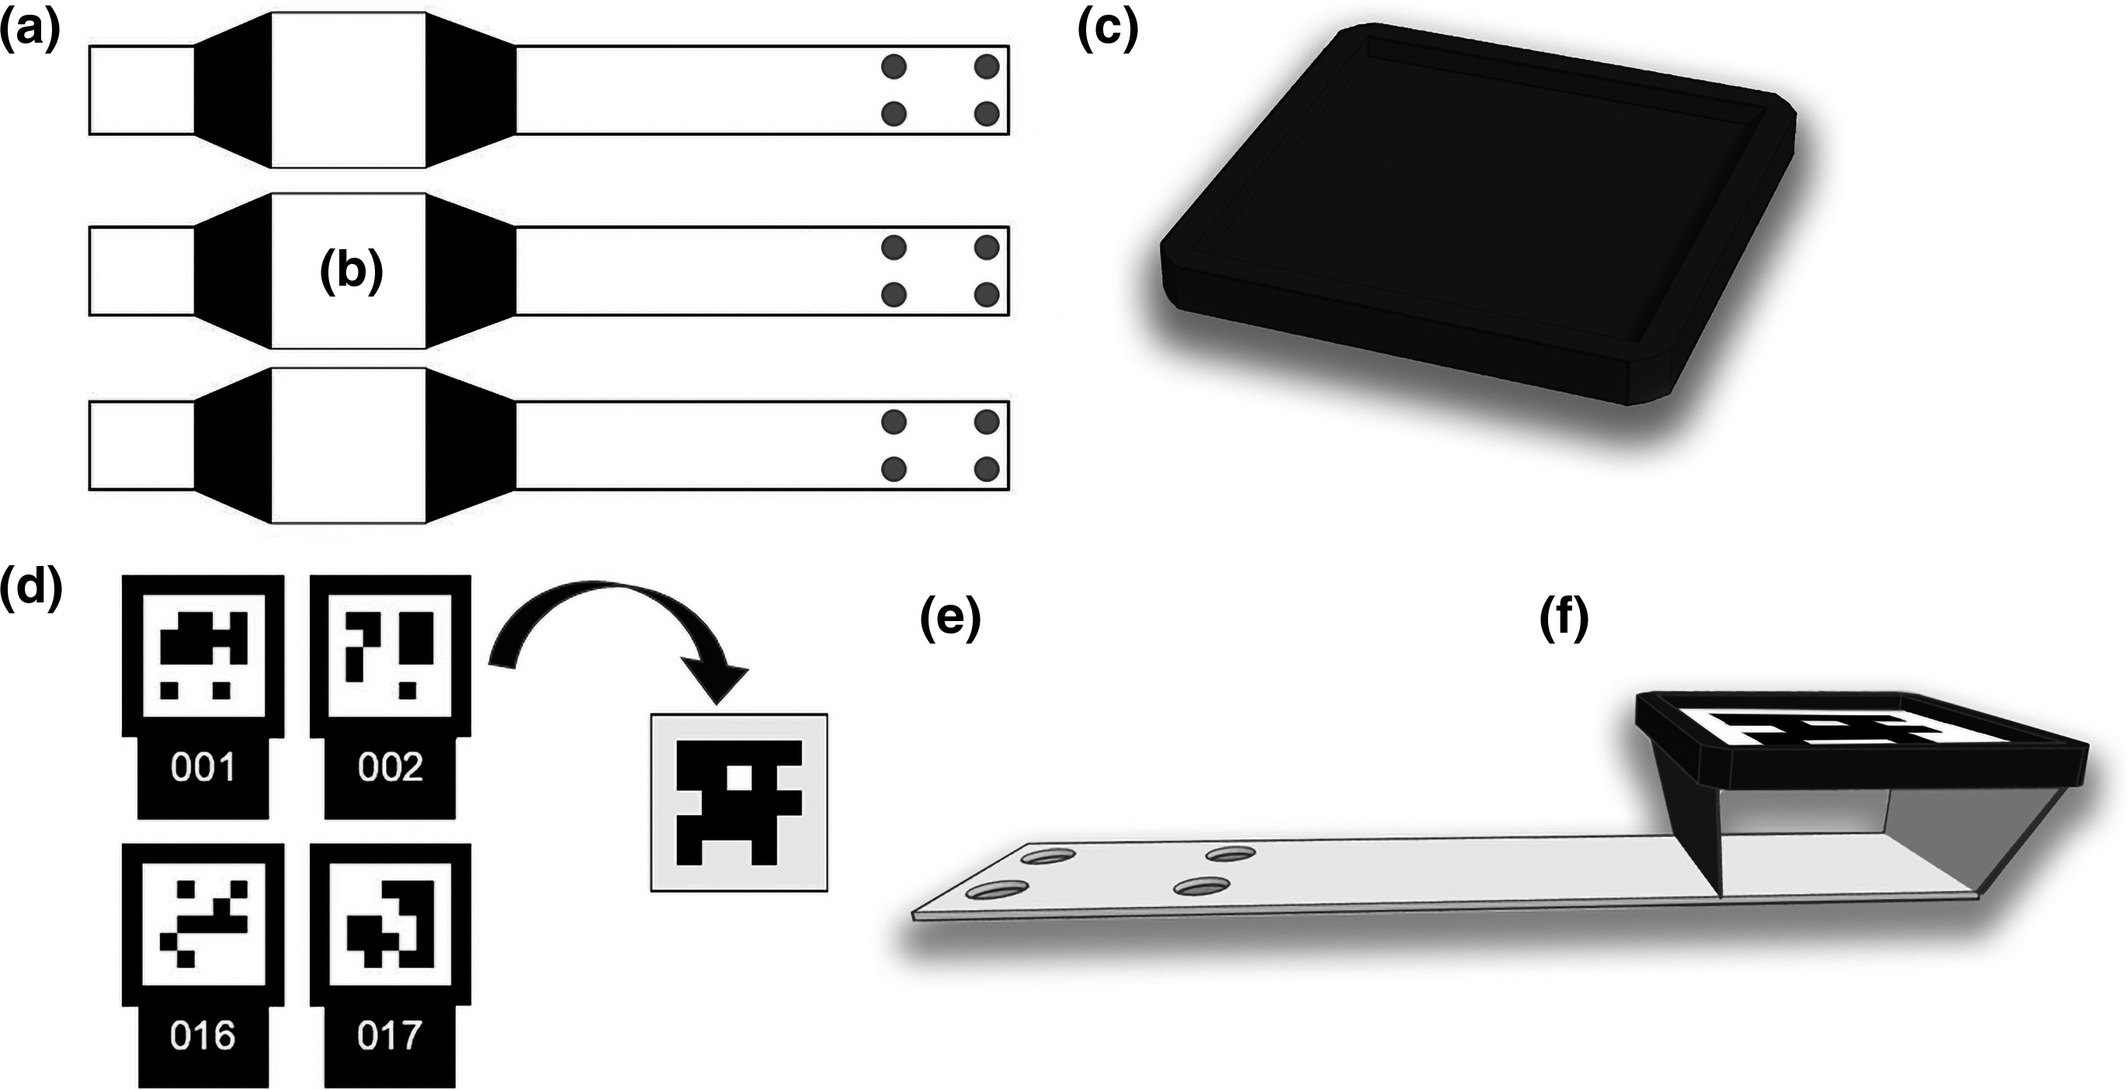
\includegraphics{Graving_IMPRS_Thesis/figures/bird_figure_1.jpg}
    \caption{Components and assembly of the backpack‐mounted barcodes. (a) Template layout. (b) Mount area where plastic trays (c) are glued. (d) Barcode layout and cutout to be glued on the tray. (e) Assembled backpack with tray and code raised on the mount (f)}
    \label{fig:bird_figure_1}
\end{figure}


Backpacks include a front strip of paper that fits between the scapulae of the bird, into which we punched four round holes (c. 1‐mm diameter, Figure 1e) to attach the elastic string that formed the straps of the backpack around the bird (Figure 2). For each backpack, we used a single piece of string 25‐cm long which we looped through the rear holes on the paper, crossed under the backpack, tied on the front holes, and kept the leads loose to allow for individual adjustment during deployment. For zebra finches, we used a 28 × 6‐mm front strip, a 10 × 10 mm mount raised 6 mm, and 10‐mm square tray. Backpacks weighed c. 0.27 g when fully assembled, including the straps.

\begin{figure}
    \centering
    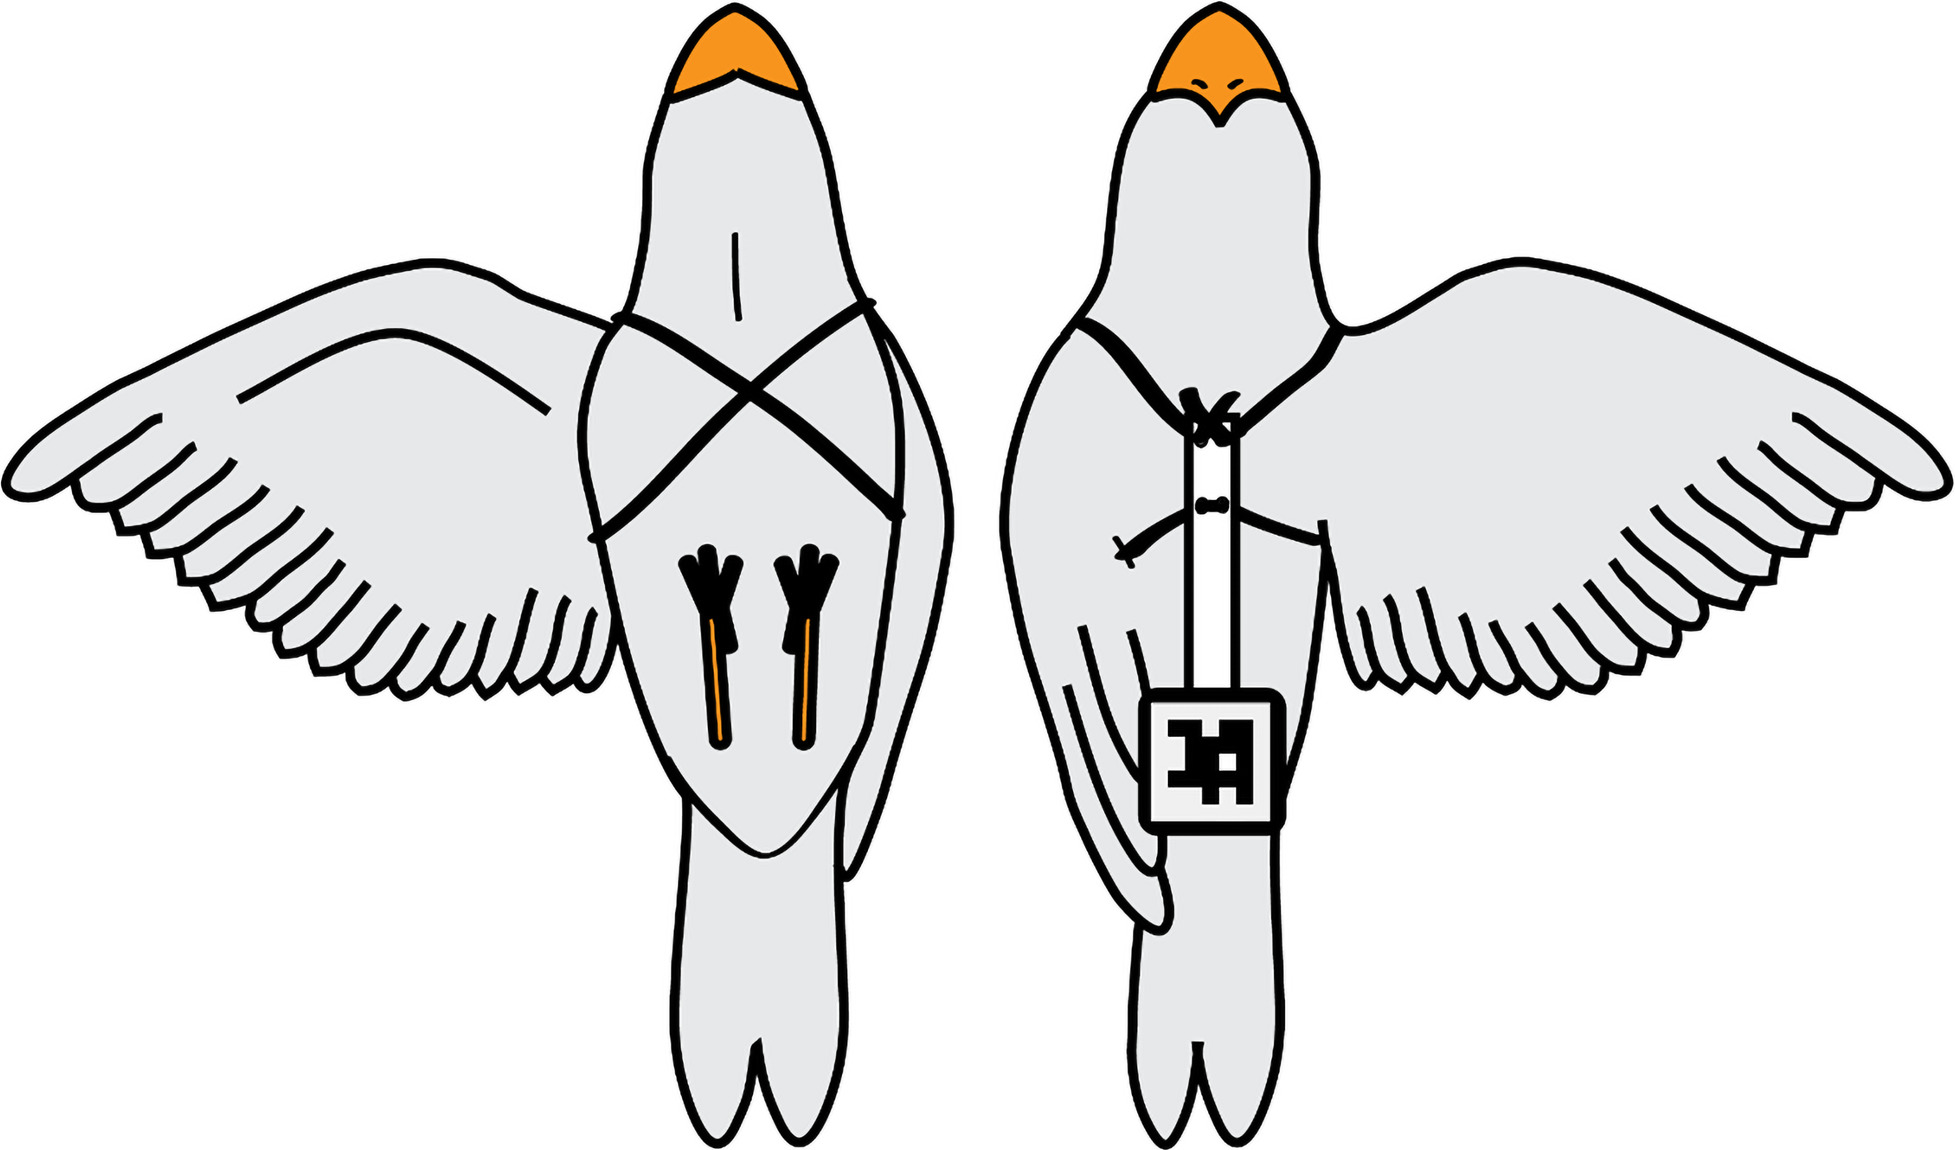
\includegraphics{Graving_IMPRS_Thesis/figures/bird_figure_2.jpg}
    \caption{Left: bottom view of bird with backpack. The string sits in front and behind the wings and crosses on the chest of the bird. Right: Top view. The string is tied at the anterior end of the backpack which goes between the scapulae, and the mount with the barcode sits on the rump, behind the wing joints}
    \label{fig:bird_figure_2}
\end{figure}
\paragraph{Backpack deployment}
The general procedure for fitting backpacks includes the following steps: (1) Catching, measuring and recording health status of each bird; (2) Backpack fitting; (3) Observation during acclimation; (4) Releasing and monitoring birds in their permanent housing; and (5) Periodic health checks.

Once we confirmed the birds were in good health (step 1), we fit a completely assembled backpack to each bird (step 2). We pre‐tied the string on the backpack with a simple slipknot and then pulled the straps over the bird's head until the front strip sat on the interscapular area, carefully pulling each wing through the looped straps. We found that the best fit was achieved when the leading edge of the raised section was below the elbow joint of the wing, and the trailing edge was above the rump (Figure 2). Once the backpack was in its final position, we tightened the string around the body, adjusting according to the size of each bird. The tightness must be firm enough to hold the backpack in position while preventing the bird to put its feet or toes inside of the loop, but also loose enough to allow the birds to fly and move freely, and to avoid blocking the crop. In their final position, the straps should sit midway between the body and the surface of the feathers. The front strip and the string loops eventually become covered by the feathers, while only the mount with the plastic tray and the barcode are visible. The mount must be positioned behind all the wing bones and joints, where only feathers can be in contact with it.

After fitting the backpacks, we placed subjects in a small observation cage (step 3) to monitor their behaviour. This step is critical for animal safety. We monitored birds for up to 1 hr until we were sure that they behaved normally, that is, with no observable hindering of movement. A well‐fitted backpack allows the animal to move freely, with no interference for flying, walking, landing or perching. Most birds tried to pull the backpacks or the straps off during this period. In our experience, the intensity and duration of this behaviour was not necessarily a signal of an ill‐fitting backpack and, on the contrary, preening helped to accommodate all the new elements. We found that the acclimation process worked better when subjects were kept in small groups (2–5) and in a separate room with no people present, as it reduced stress and allowed for allopreening, feeding and undisturbed movement. Once we considered the deployment procedure was successful, we made a final check of the adjustments, secured the knot near the neck of the bird a second small knot and cyanoacrylate glue, and cut any excess string from the leads. When necessary, we also trimmed some covert feathers around the mount to prevent any obstructions on the codes that might hinder detection.

Every time we observed a bird with hindered movement or unusual behaviour that could be related to the backpack (i.e. foot or toes trapped in a loose strap, incapable of flight, or unbalanced perching), we checked and readjusted the straps using blunt‐tip tweezers. In some cases, if a bird's movement did not improve after the adjustment, we completely removed the backpack, let the bird rest to reduce stress, and observed it without the backpack before trying another deployment. After a second attempt, a few birds (4 of 58) still showed suboptimal performance despite having a well‐fitted backpack and appearing to be in good health. Our testing suggests that fewer than 5\% of subjects will never acclimate to the backpacks.

\paragraph{Backpack monitoring}
We monitored the birds regularly, either during our experiments or during care‐taking activities, and constantly looked for unusual behaviour. This monitoring is important to prevent injuries or detect early symptoms of health issues, either related to the backpacks or otherwise. In our experience, most of the signs that could suggest ill‐fitted tags occurred within the first 2 days of observation after deployment and were addressed promptly. Importantly, some issues were only detectable when birds were settled in their permanent housing environment where they could fly much more extensively. We also monitored the birds by assessing the tracking data to identify individuals that were outliers in the number of detections (suggesting they behaved differently to others). The main issue we found arose after release into large aviaries was the backpack rubbing on the body or wings of the bird. Symptoms of this included bald spots on wings or neck, reduced movement or difficulty flying. These were addressed immediately by ensuring the backpack mount (and tray) were correctly fitted (i.e. not crooked and positioned away from the wings). However, in some cases, when the problem persisted, we completely removed the backpack, let the bird rest, and observed its behaviour without the backpack.

\subsubsection{Camera systems}
Barcodes can be detected using either photos or video. The choice largely depends on the research question to be addressed, as well as the scale of data collection and its associated processing and storage requirements. In this section, we provide details on the necessary considerations for implementing a camera system, and details of our experience using several implementations, including high‐resolution photos and video from action cameras, computer‐controlled DSLR cameras and the programmable camera module for the Raspberry Pi. We also discuss the pros and cons of each system for different types of research questions.

\paragraph{Code size and capture}
For adequate detection and recognition of individual birds in photos or videos, the size of the barcodes should be at least 20 pixels per side in the captured image data (Crall et al., 2015), but this can vary depending on tag design and camera hardware. Detectability of tags can be improved, using high‐resolution cameras, reducing the distances between the codes and the camera (either physically or by using zoom lenses), or increasing the physical size of the deployed tags (which is limited by the study organism). Other considerations such as lens distortion, sharpness, and depth of field must be considered depending on the setup and area being captured. Lens distortion can be partially corrected via software, but this correction reduces the effective resolution of the images, especially for wide‐angle lenses (Figure 3). Depth of field is an important consideration if the birds can perch at different heights, although issues can be avoided by having all perches on the same plane. Finally, the camera shutter speed needs to be chosen carefully. Slow shutter speeds result in blurred or overexposed codes and, thus, failed detections. To prevent these problems, exposure time should be set as short as possible while ensuring that contrast and noise levels are adequate for the software to successfully read the codes. We found that darker images had greater detectability as they increased the clarity of the edges within the barcodes by reducing bleeding of the white areas of the barcode into the black areas.

\begin{figure}
    \centering
    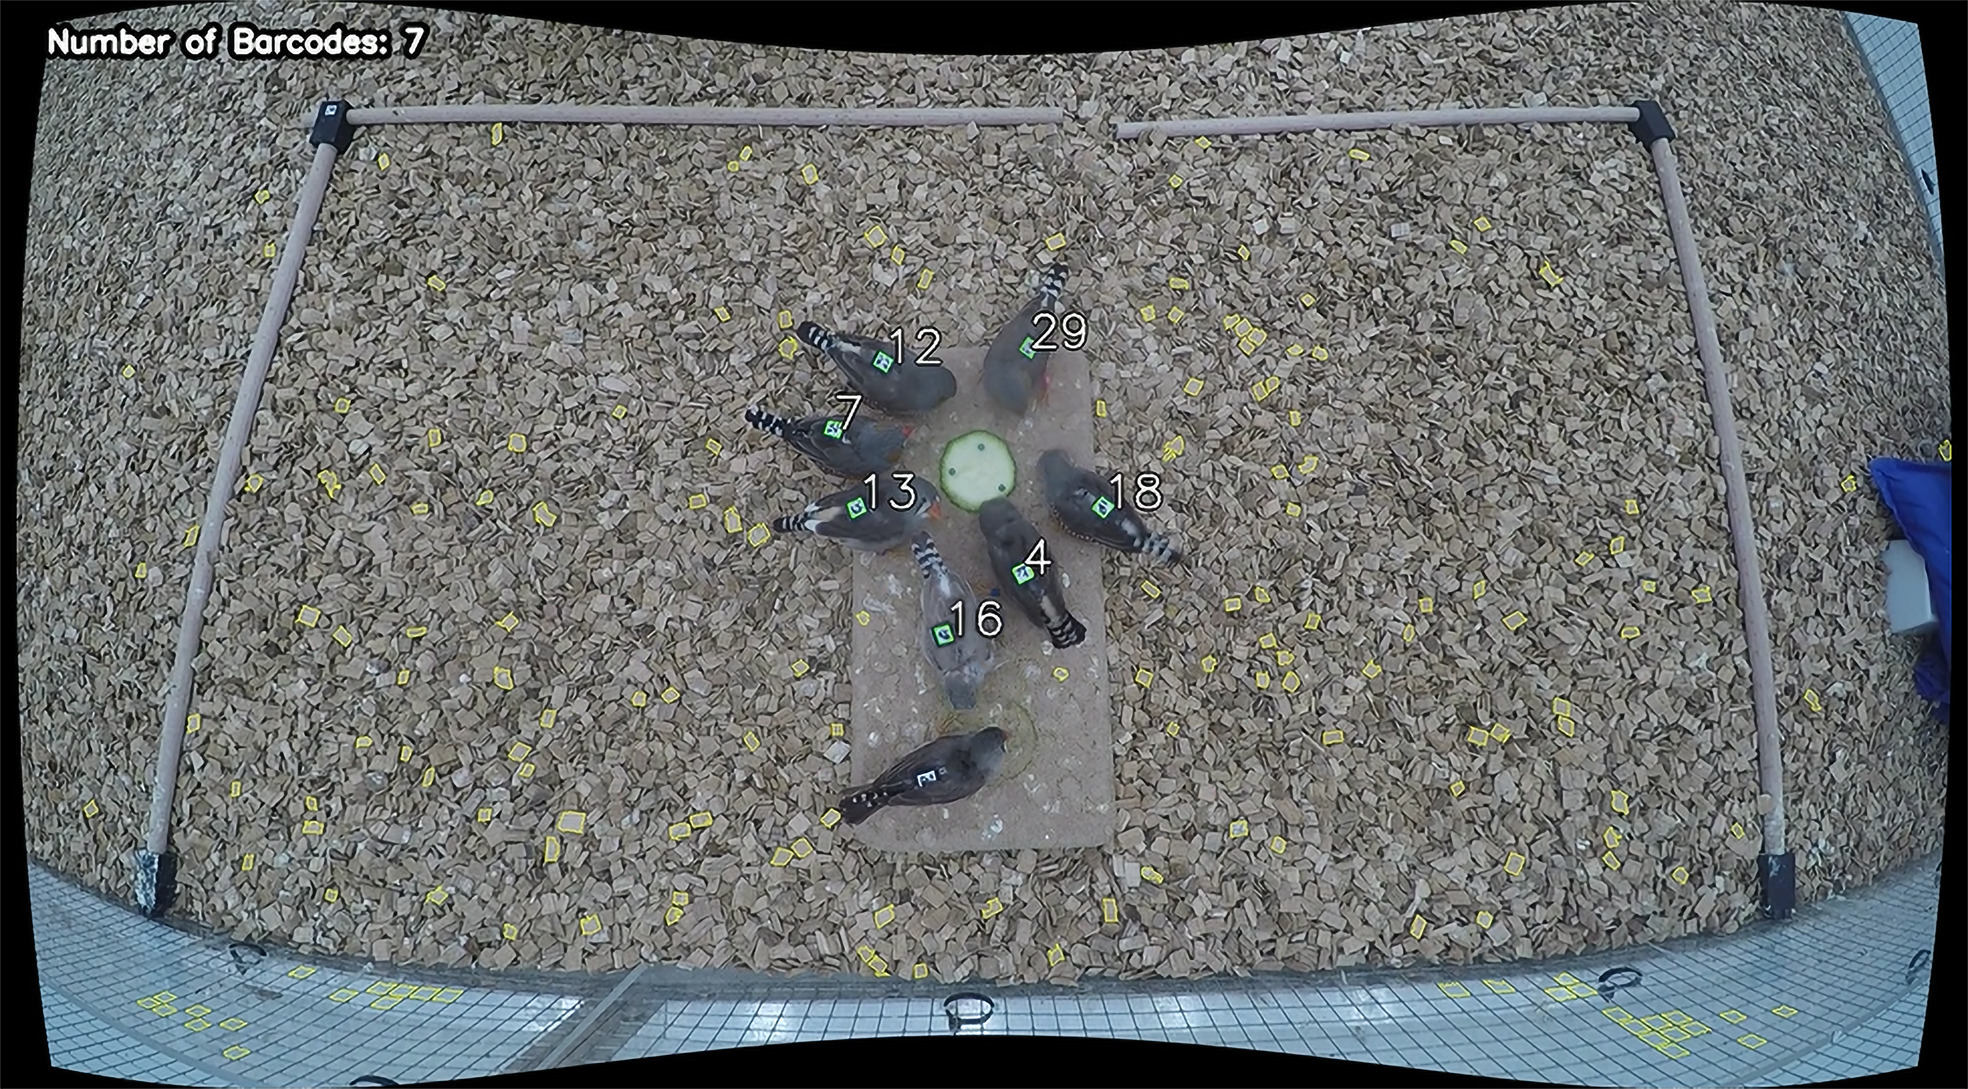
\includegraphics{Graving_IMPRS_Thesis/figures/bird_figure_3.jpg}
    \caption{Barcode detections in a feeding context in one video frame (from a GoPro camera). The food source in the centre of the arena was pinned to a wooden board to prevent birds from moving it out of the frame. The tracking algorithm detected barcodes on the back of each individual despite being on a complex background (wood chips). The yellow polygons are objects that were detected as candidate barcodes but did not match any known identities. The bird near the bottom of the image was not detected because its wings covered the barcode in this frame. Individual 16 was oriented away from the food. The black edges around image illustrate the software correction we used to partially compensate for wide‐angle lens distortion
}
    \label{fig:bird_figure_3}
\end{figure}

\paragraph{Photos or video?}
Imaging technology requires a trade‐off between spatial and temporal resolution as hardware is always limited in its capacity to transmit and process signals. The choice between using photos or videos when capturing image data depends on the spatial or temporal resolution required to answer the research question. Video offers higher temporal resolution (typically ≥24 Hz) at the expense of spatial resolution (most hardware is limited to 3,840 × 2,160‐pixels), making it more suitable for studying behaviours that occur over short periods of time and in confined areas (e.g. allopreening, aggressive interactions, mating displays or copulation). Photos offer increased spatial resolution (>50 megapixels for some DSLR models) at the cost of temporal resolution (most cameras are limited to <15 Hz at full resolution), making them ideal for assessing behaviours in larger, open areas that do not require high‐frequency measurements (e.g. feeding, bathing, co‐perching, co‐feeding, etc.) and for quantifying associations over longer timescales (i.e. social networks, pair formation, etc.). Current imaging technologies vary widely in frame rate, image resolution, and file sizes, and different camera setups can be adapted for data collection depending on the research question and project budget. We implemented and tested three types of recording devices.

\paragraph{Action cameras}
We used GoPro Hero 4 action cameras to record video of the birds in a feeding arena 90 × 50 cm on the floor of the aviaries (Figure 3). We set the cameras to run continuously until the battery was depleted (c. 45 min) and chose a resolution of 1,920 × 1,080 pixels (1,080p) at 24 Hz to limit file size, reduce processing time, maximize battery life, and prevent the camera from overheating. We created a 3D‐printed arm to attach the camera to the side of the cage, 50 cm above the feeding arena and manually started recordings immediately after providing birds with a high‐value food patch (to attract them to this focal area of the camera).

These cameras produced adequate image quality but had noticeable distortion due to the wide‐angle fixed lenses. We manipulated the resulting images to reduce distortion before running the detection code (see “extracting data from images”). At 1,080p, we observed that the codes were sharp enough for detection, although at 24 Hz some frames suffer from image blurriness when birds moved. At 1,080p resolution, we generated a 4‐GB file every 15–17 min of video, which is the maximum file size supported by the cameras. This means that in a 45‐min recording session, we had to process three videos and store at least 12 GB. Limitations of this setup include the need to manually operate the cameras, restricted recording time due to battery life or large file size, and limited options for automating the entire system. Some of these problems, such as limited storage, lens distortion, and lack of automation, have been mitigated in newer models of the GoPro Hero series, as well as other brands of action cameras.

\paragraph{Digital SLR cameras}
We briefly tested data collection using four Canon EOS1200 DSLR Cameras with 18–55 mm lenses for recording video or still images. We connected these cameras to Raspberry Pi 3 single‐board computers to control the image capture frequency. We placed the cameras at the top of the aviaries facing directly down. The cameras were set to capture one image at 1/200‐s every 10 min to measure the position of birds sitting on perches made from natural branches. These cameras can deliver high quality images up to 5,184 × 3,456 pixels (18 megapixels) and the zoom lenses allow for easy accommodation to different distances and to cover either small or large areas. However, this model had a loud mechanical shutter, which visibly disturbed the birds in the enclosed aviary space. Rather than modifying or removing the shutters, we abandoned this setup in favour of cameras with electronic shutters and no moving parts. In video mode, DSLR cameras can record high‐resolution video (1,080p) which is sufficient for collecting detailed movement data. Unfortunately, the recording time for many models is limited to 30 min.

\paragraph{Single-board computers with camera}
We used Raspberry Pi 3 Model Bs (Raspberry Pi Foundation), each fitted with an 8‐megapixel Camera Module V2 (RS Components Ltd and Allied Electronics Inc.), to record photos of birds on perches (Figure 4). We installed two of these on top of each aviary, covering most of the perch system without overlap. To record the birds present, we set the system to capture one image every 10 s, from dawn to dusk. In our experience, one of the most important advantages of this system is the possibility of programming automation scripts via the picamera software package (Jones, 2013) for Python (Python Software Foundation, available at http://www.python.org). This approach gives the user fine‐scale control over the quantity, sampling frequency, and spatial resolution of photos and videos. In combination with standard networking protocols like Secure Shell, these features allow for a fully automated pipeline that includes image capture, with file transfer, processing, and data storage when networked to a more powerful host computer. Another important advantage of these computers is their low cost, especially if the system requires multiple cameras per aviary or across multiple replicas in an experimental setup. Among the disadvantages of this system is the inconsistent quality of the camera modules (a small proportion of our cameras were unable to produce sharp images). To deal with this, we tested the cameras on the experimental setup and avoided using those that seemed to be defective. Although these camera modules provide a large depth of field, they require manual focusing, which can be difficult and is often inconvenient (Table 1).

\begin{figure}
    \centering
    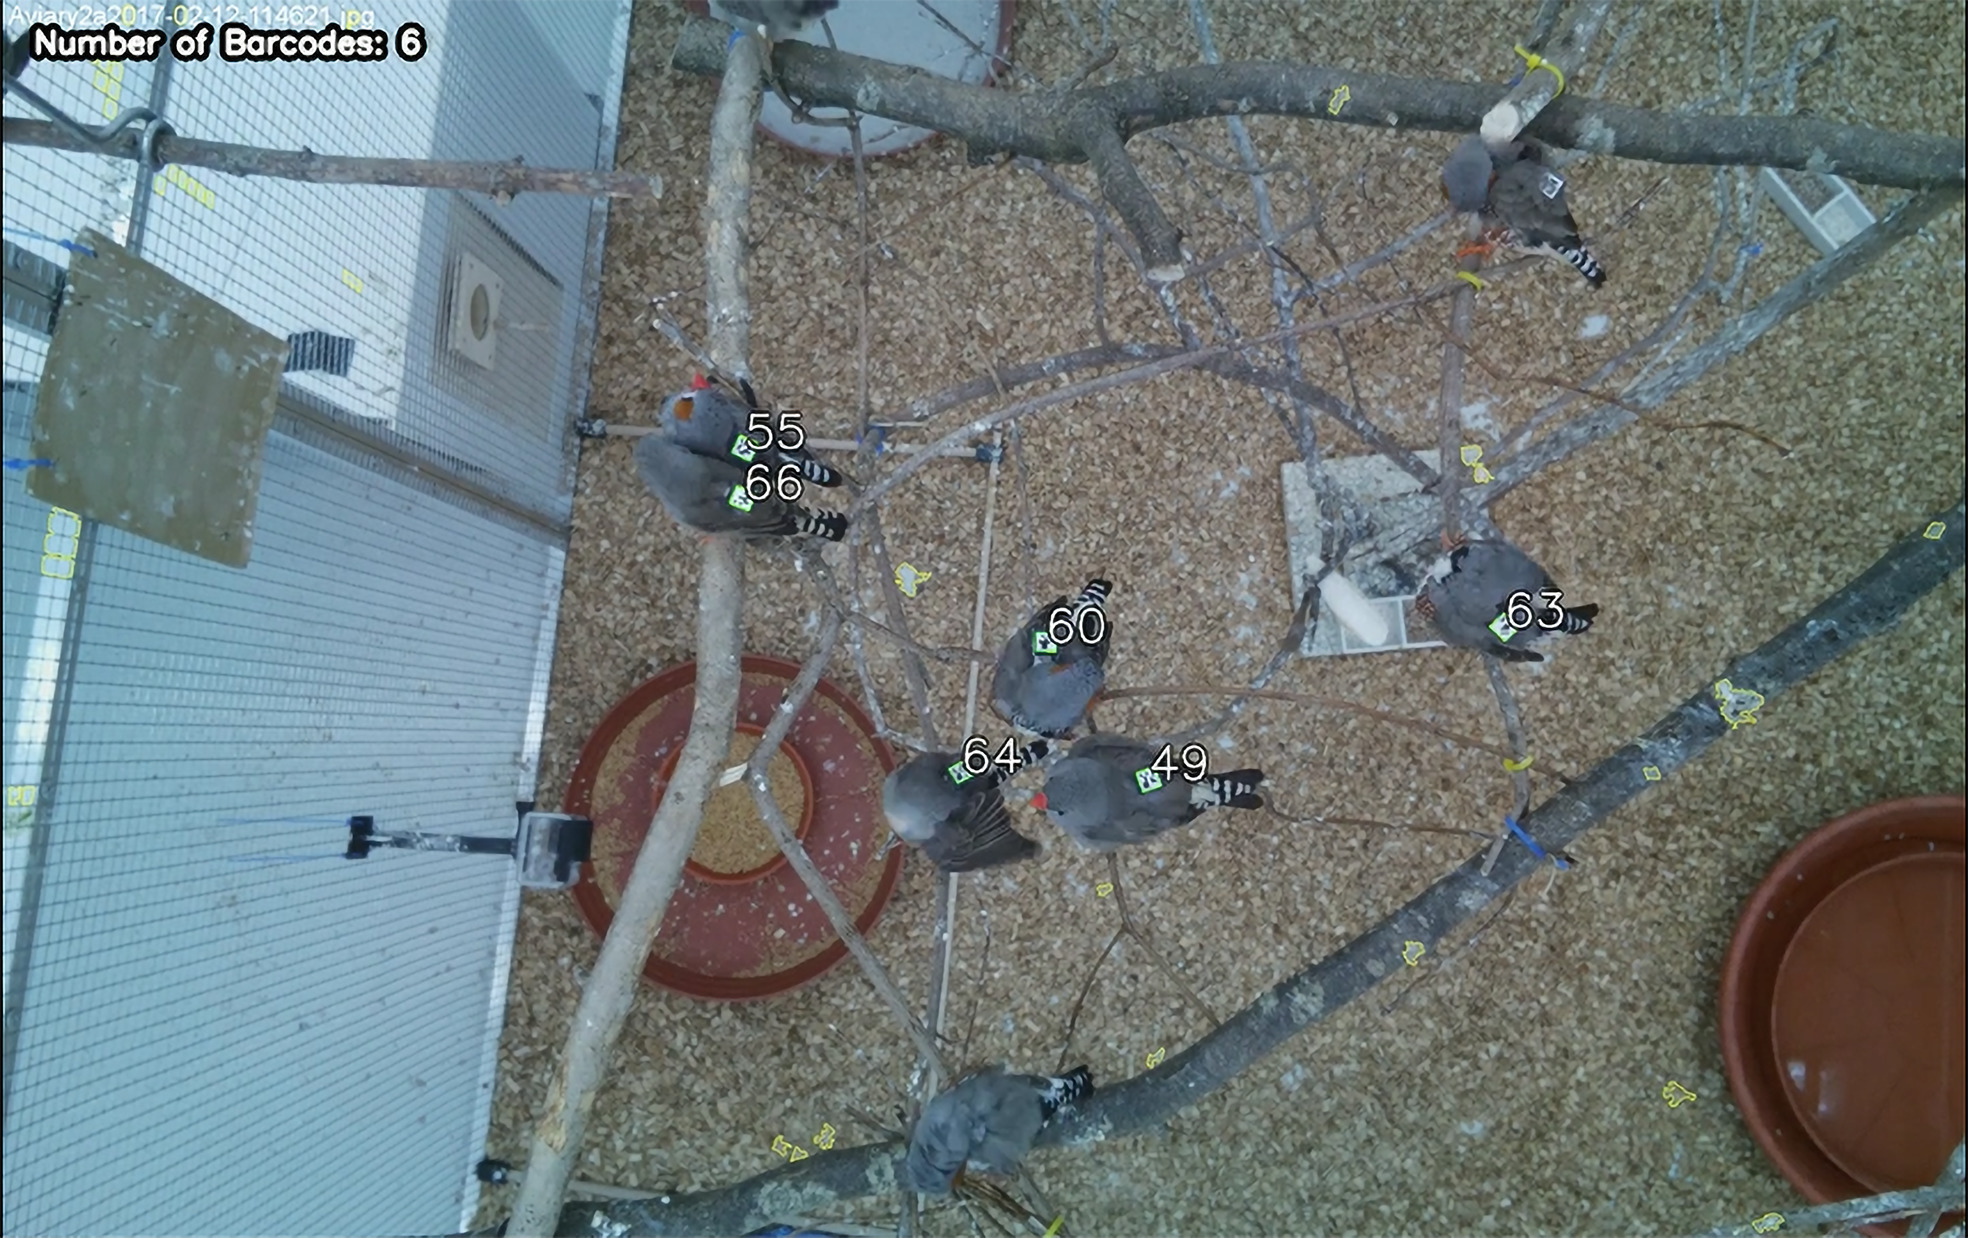
\includegraphics{bird_figure_4}
    \caption{Barcode detections in a social perching context (photographed with the Raspberry Pi camera module). The software can easily detect visible codes in complex aviary environments and extract information about important interactions, such as direct body contact (individuals 55 and 66), that many tracking algorithms would fail to detect
}
    \label{fig:bird_figure_4}
\end{figure}
\begin{table}
\caption{Summary of the pros and cons of different camera implementations tested}
    \begin{tabular}{| m{0.2\textwidth} | m{0.4\textwidth} | m{0.4\textwidth} |}
         \textbf{Camera system} & \textbf{Advantages} & \textbf{Disadvantages} \\ \hline
         DSLR (Canon EOS 1200)	& Image quality. Availability of lenses and accessories. Suitable for video or photo. Low‐light performance.	& Noisy mechanical shutter (this model). Video limited to 30 min. Bulky. Costly. \\ \hline
         Action Cameras (GoPro Hero 4)	& Compact size. Image resolution and quality. Suitable for video or photo. Wide angle lens suitable for small spaces.	& Lens distortion. Limited battery life. No display (this model). Manual operation (this model). \\ \hline
         Single‐board computers/Camera module (Raspberry Pi 3 Model B with Camera V2)	&
         Inexpensive. Compact size. Suitable for video or photo. Programmable. Network access. Expected improvements and software updates. No battery life limitation.	& Lower image quality. Fixed recording area. Difficult manual focusing.
    \end{tabular}
\label{table:bird_table}
\end{table}

\subsubsection{Extracting data from videos and images}
Once videos or images are recorded, the next step is to extract location data from the barcodes contained in the image data. Several software libraries are available to accomplish this (Crall et al., 2015; Garrido‐Jurado, Muñoz‐Salinas, Madrid‐Cuevas, & Marín‐Jiménez, 2016; Graving 2017; Wang & Olson, 2016), and each provides its own set of barcodes. These software libraries all extract the identity, location, and orientation of each tag from image data. In our study, we used the software library pinpoint by (Graving 2017), which is a based on the work of Garrido‐Jurado et al. (2016).

\paragraph{Code detection}
The detection algorithm finds the identity matrix of the barcode using the contrasting white and black edges between the barcode and the black frame of the plastic tray on the backpack. Images are binarized using an adaptive (spatially localized) thresholding algorithm, which allows for uneven lighting, and candidate barcodes are detected based on their geometry, which allows for complex backgrounds. Once a candidate barcode is detected, the identity matrix is extracted from the pixel data and compared to known identities stored in a tag dictionary. The tracking algorithm can reliably detect the codes at arbitrary angles, even when they are not completely perpendicular to the central‐axis of the camera lens. The software provides the identity and Cartesian coordinates for the corners of each detected barcode with sub‐pixel resolution, which can be used to calculate the orientation of the code (note the importance of fitting the code in the right direction on the birds).

\subsubsection{Example data analyses}
To briefly demonstrate the use of this automated approach to data collection and analysis, we studied the foraging behaviour of individual zebra finches at a high‐quality food source and constructed foraging networks based on high‐resolution movement data measured using our system. Social networks are particularly challenging to study using manual observation because they require measuring the behaviour of most or all individuals simultaneously. To achieve this, we created an arena 90 × 50 cm on the floor of each of the two aviaries and provided birds with an ephemeral high‐quality food resource (a slice of zucchini/courgette) twice per day (around 9.00 and 16.00 hr). We used a barcode to record the centroid of the resource, which was subsequently removed to allow birds unobstructed access to food. Birds were fasted for an hour before the experiment to ensure they were motivated to feed, and their access to the food resource was captured on video using the GoPro Hero 4 camera fitted 50 cm above the food (see above). We collected data on the two aviaries for 58 days, between December 15, 2016 and March 29, 2017.

We extracted feeding association data, representing the propensity for individuals to synchronize their feeding and tolerate one another at the food source. We recorded the identity of individuals detected at the food for every video frame by defining a feeding zone with respect to the centroid of the food resource. A feeding event was recorded when a barcode was detected within a 154‐pixel (or c. 8‐cm) radius of the resource centroid, and the bird was facing the food (i.e. the centroid was within the 180° zone in front of the bird) (Figure 3). Once we identified the individuals in every frame and classified feeding events, we constructed a weighted, undirected social network representing the co‐feeding relationships among individuals (represented as nodes) in each flock. We accomplished this by transforming our data into a matrix of pairwise associations using a simple ratio index ($\mathrm{SRI}$) for every pair of individuals in each flock (see Farine & Whitehead, 2015). Here, the edge weight between two individuals ($\mathrm{SRI}_{ij}$) is the probability of observing individuals $i$ and $j$ feeding together given that either $i$ or $j$ has been detected. This calculation is simply given by the following:
\begin{equation}
    \mathrm{SRI}_{ij} = \frac{x_{ij}}{n},
\end{equation}

for $i, j = 1, \dots, N$ and $i \neq j$, where $N$ is the total number of individuals in the flock, $x_{ij}$ is the number of frames in which individuals $i$ and $j$ were feeding together, and $n$ is the total number of frames where either $i$ or $j$ was detected (alone or together).

\subsection{Results}
\subsubsection{Barcode deployment and maintenance}
We deployed backpacks on 58 zebra finches (Figure 5), which required about 3 min of handling per individual, plus observation and monitoring time. All the deployed backpacks lasted throughout the experimental period (4 months or more) without causing any injuries to the birds. However, minor maintenance was required as backpacks and codes showed some wearing due to grooming and allopreening (see backpack‐mount in Figure 5). Common issues included loss of ink on and around the barcodes, weakened paper around the front holes, and unglued mounts. We also noticed that, in a few cases, the straps lost elasticity after 4 months and appeared loose. More commonly, we observed that debris (i.e. food remains or excrement) on the barcode obstructed its detection. Every time we detected one of these issues, we addressed it immediately to guarantee both safety of the birds and quality and continuity of the data collection. For any minor issues, we carefully cleaned the codes to remove debris, or covered the ink‐less spots with black ink permanent markers. For extensive damage on the mount or the surface of the barcode, we removed and replaced the mount keeping the strip and the elastic string on the bird, thus reducing manipulation and acclimation time. In cases that required a whole new backpack, we repeated the process of the first deployment.

\begin{figure}
    \centering
    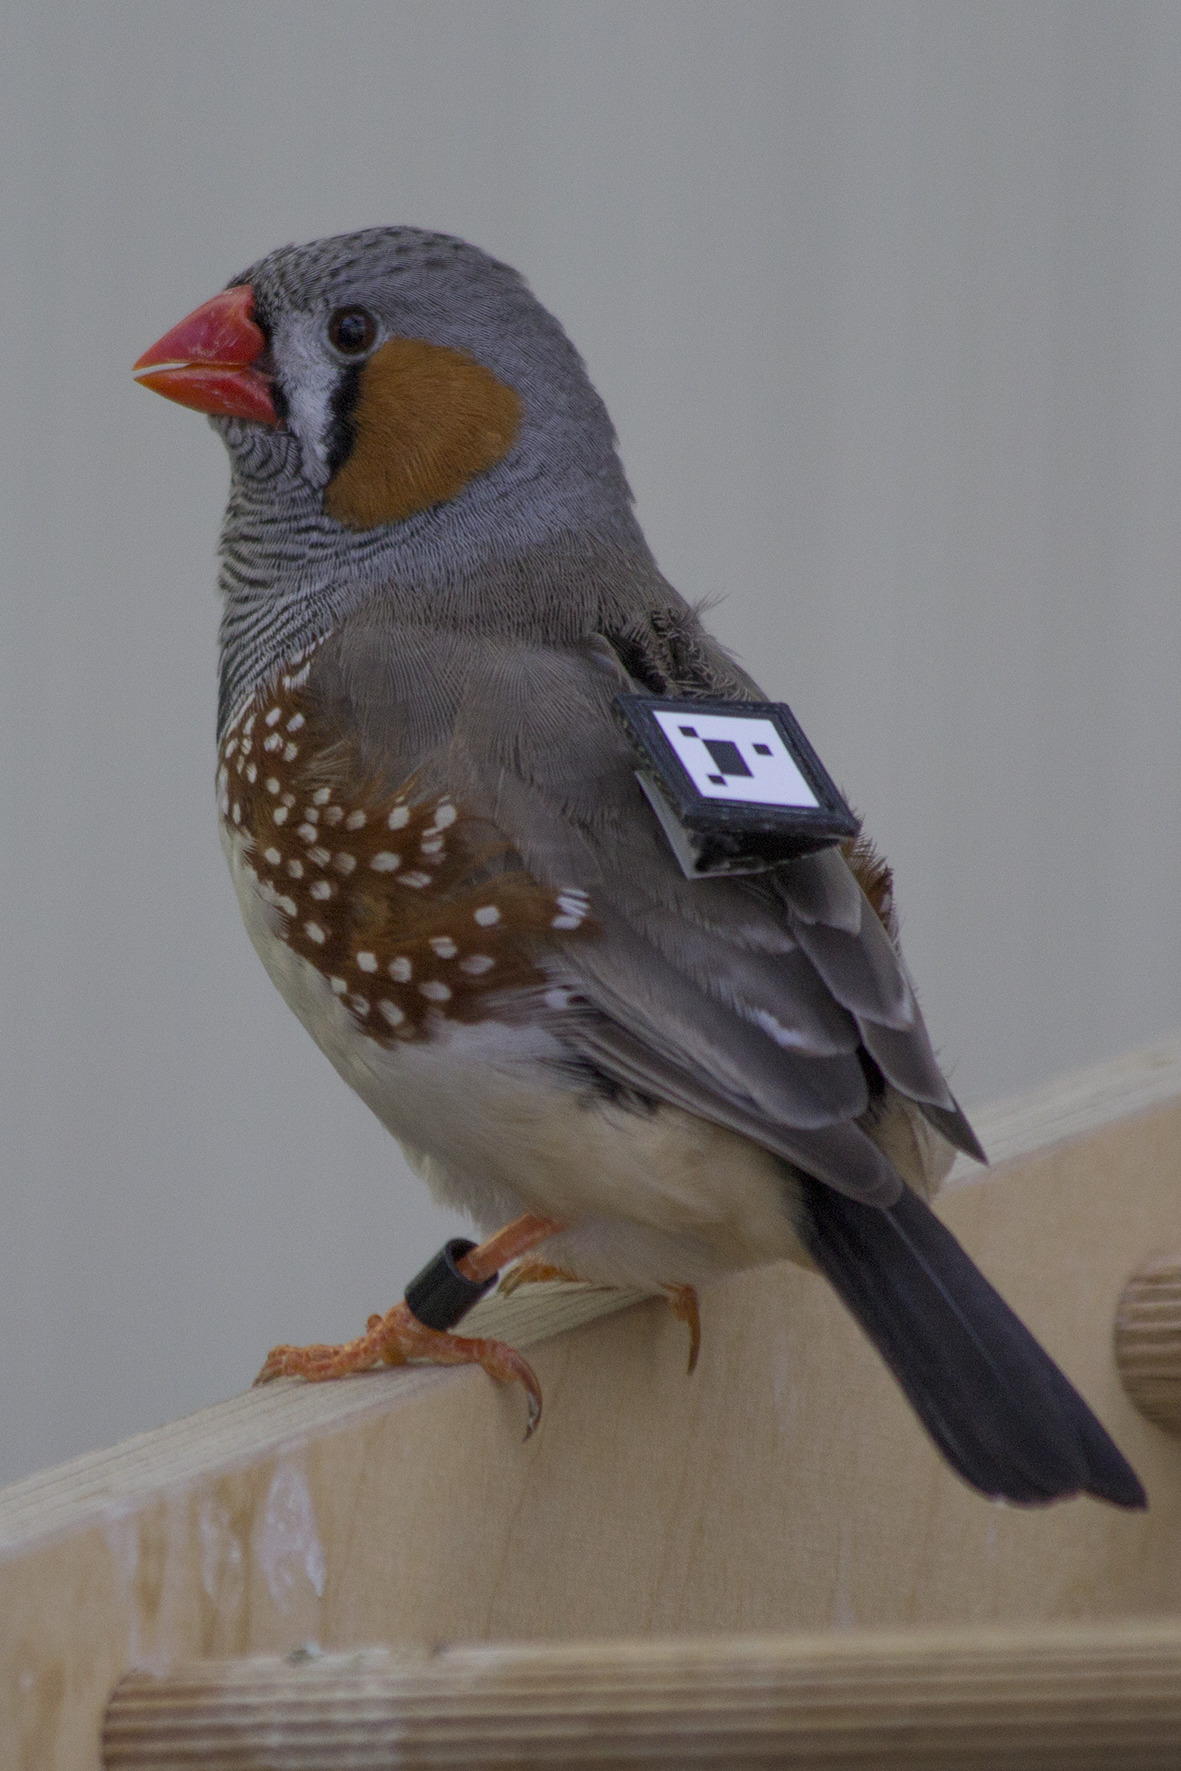
\includegraphics{Graving_IMPRS_Thesis/figures/bird_figure_5.jpg}
    \caption{Male zebra finch with a barcode backpack c. 4 months after fitting. Note the wearing on the backpack structure caused by grooming behaviours
}
    \label{fig:bird_figure_5}
\end{figure}

\subsubsection{Detection}
We recorded 48 hr of video at the feeding arenas using GoPro Cameras and recorded photos using Raspberry Pi cameras. The detection software identified 52.05\% of the barcodes (i.e. birds) present in 100 randomly selected frames from the GoPro footage. This percentage was improved to 64.58\% after simple linear interpolation of positions across short gaps of missing data (e.g. 1–24 frames of video). From the photos of birds perched on the aviary branch system, the software detected 60.4\% of the individuals present in 100 randomly sampled images captured, using the Raspberry Pi cameras. The most common reasons for failed‐detections were motion blur and feathers temporarily obscuring parts of the code (e.g. Figure 3). Motion blur was most prominent in GoPro videos but is easily prevented in photos using shutter speeds of 1/1000‐s or faster (which can even identify birds in flight, Figure 6). Trimming some feathers around the code during backpack deployment can increase the number of detections, although we expect the current rate of data collection to be sufficient for most applications and research questions.

\begin{figure}
    \centering
    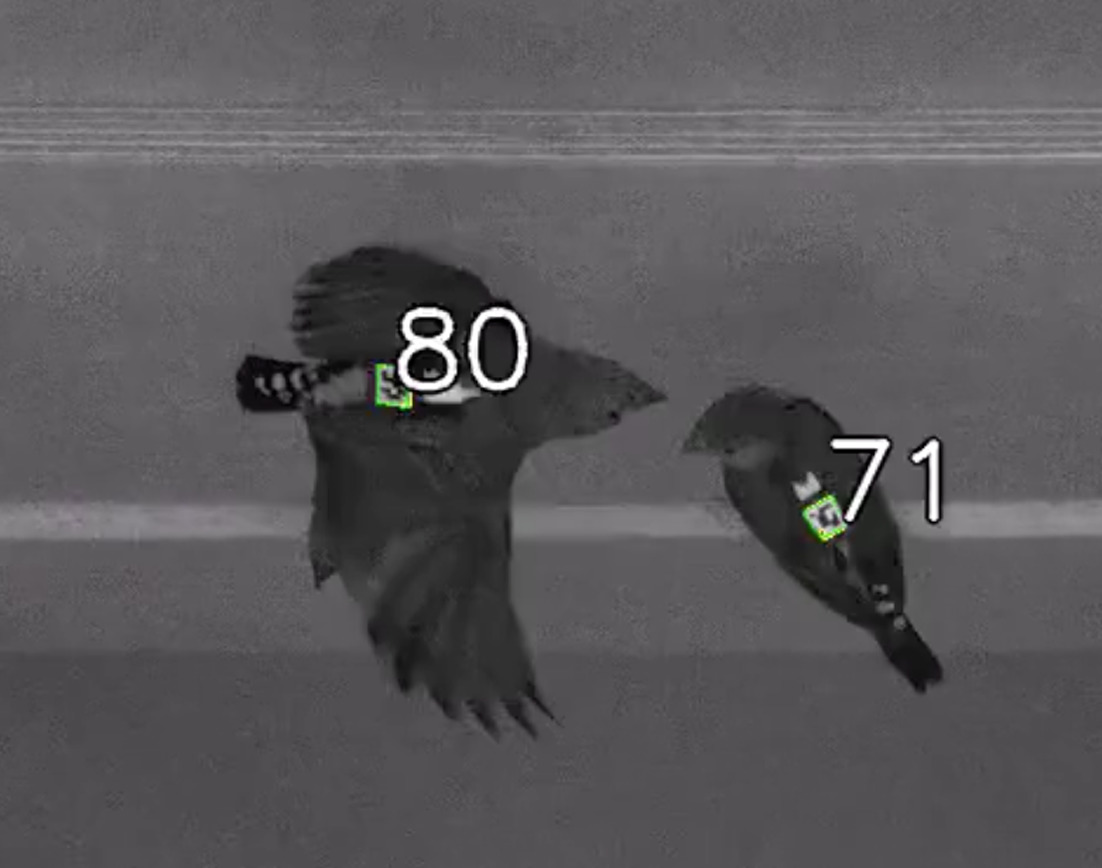
\includegraphics{Graving_IMPRS_Thesis/figures/bird_figure_6.jpg}
    \caption{Example of a zebra finch (individual 80) being detected in flight (with 1/2000‐s shutter speed)
}
    \label{fig:bird_figure_6}
\end{figure}
\subsubsection{Example data analyses}
Using image data collected with a GoPro mounted over the food arena, we were able to distinguish birds consuming the resource from those present in the frame but not feeding (Figure 7). For example, from a single 45‐min observation period, as shown in Figure 7, we recorded 74,960 records of individual positions. These records also contain many potential interactions. We demonstrate that the data on the co‐presence of individuals at a food source can be used to generate social networks (Figure 8), a powerful approach used in many studies of animal behaviour for which extensive observation data are required.

\begin{figure}
    \centering
    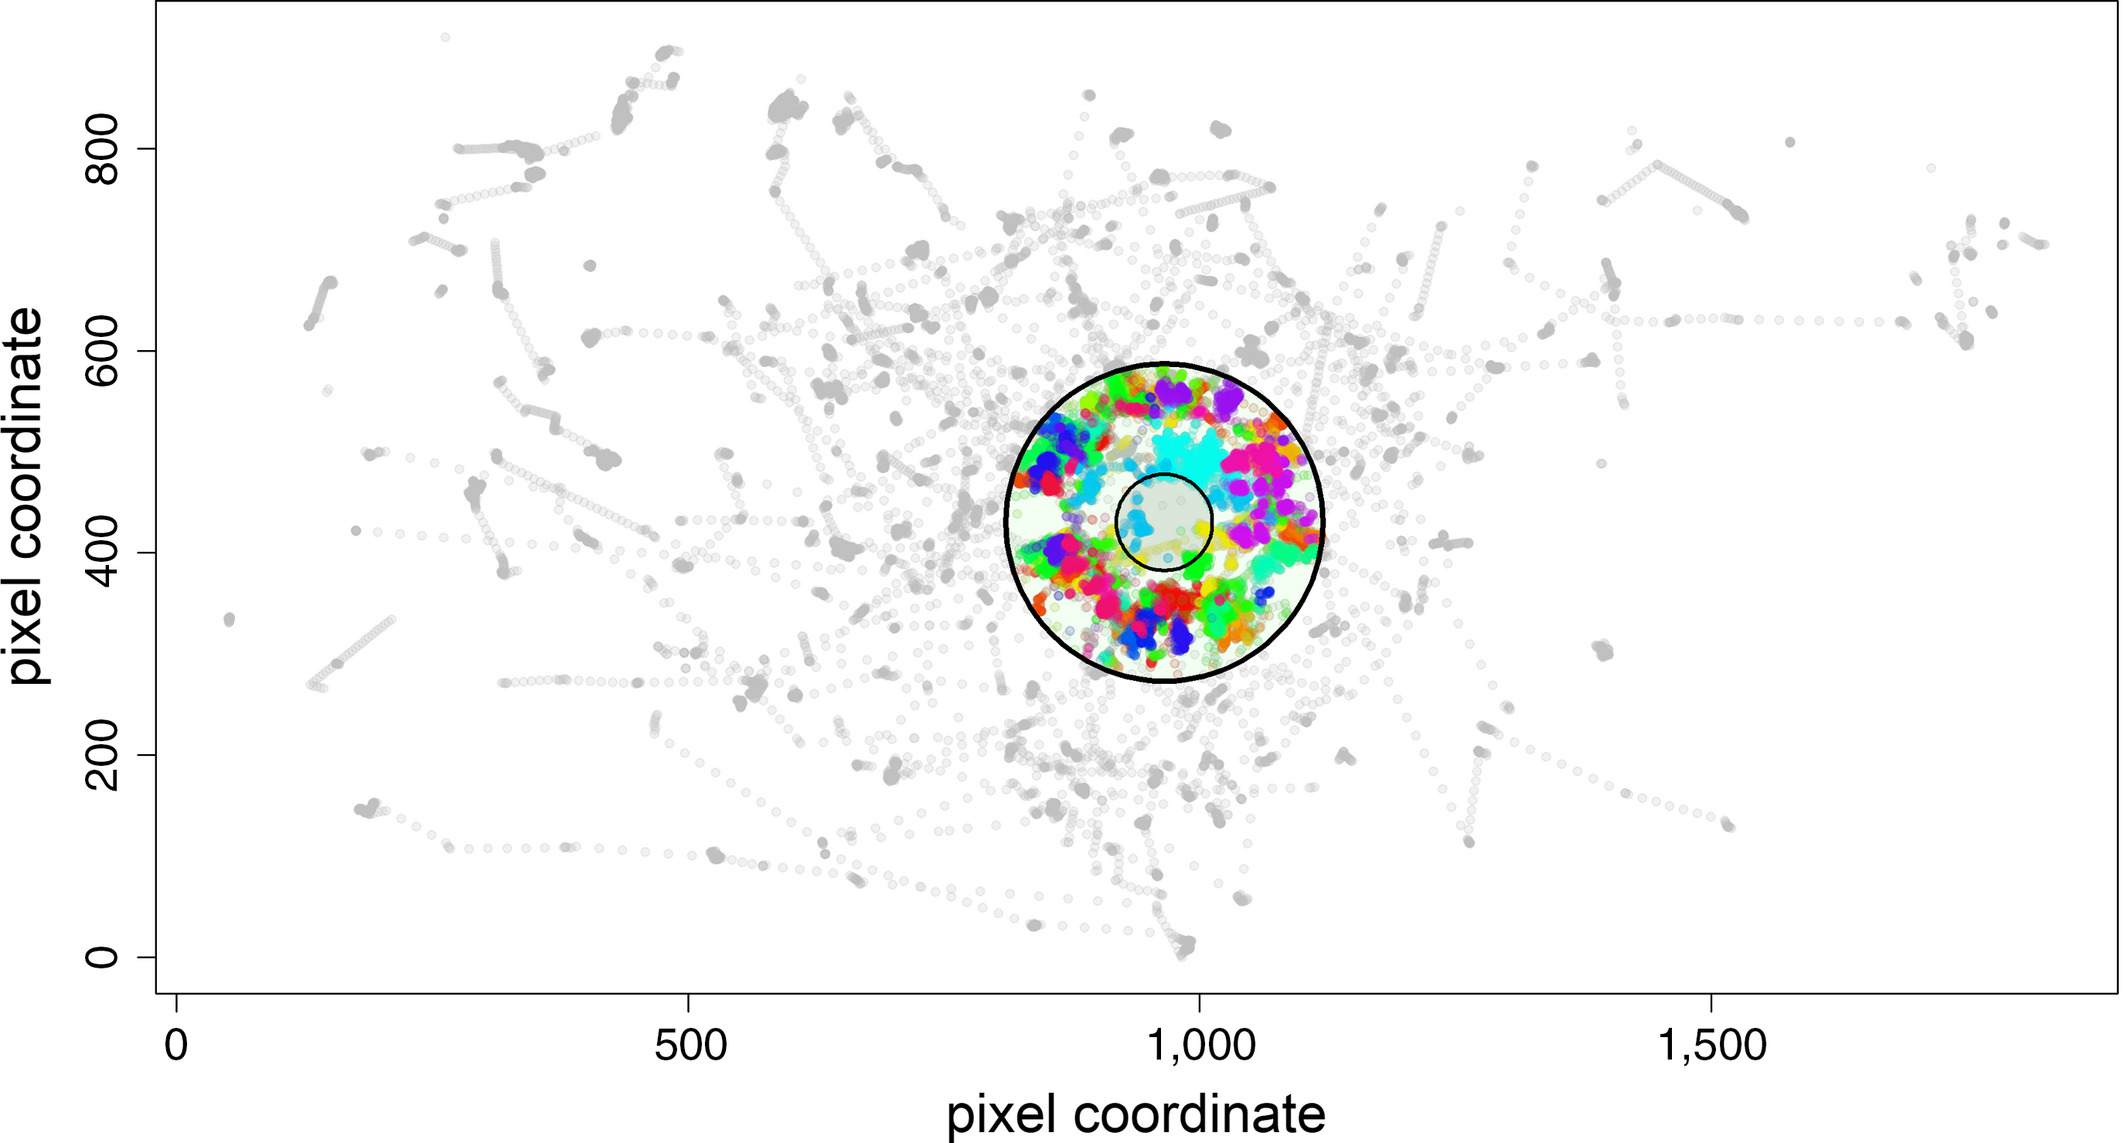
\includegraphics{Graving_IMPRS_Thesis/figures/bird_figure_7.jpg}
    \caption{Detection of feeding behaviour characterized by proximity and directionality to the food source. The inner circle represents the outline of the food source, and the outer circle represents the 154‐pixel boundary for birds to considered to be “at food.” Coloured dots represent detections of different individuals within the “at food” zone. Grey dots are birds present and identified in the frame but not actively feeding. The positions of birds away from the centre of the frame are less accurate due to lens distortion (see Figure 3)
}
    \label{fig:bird_figure_7}
\end{figure}

\begin{figure}
    \centering
    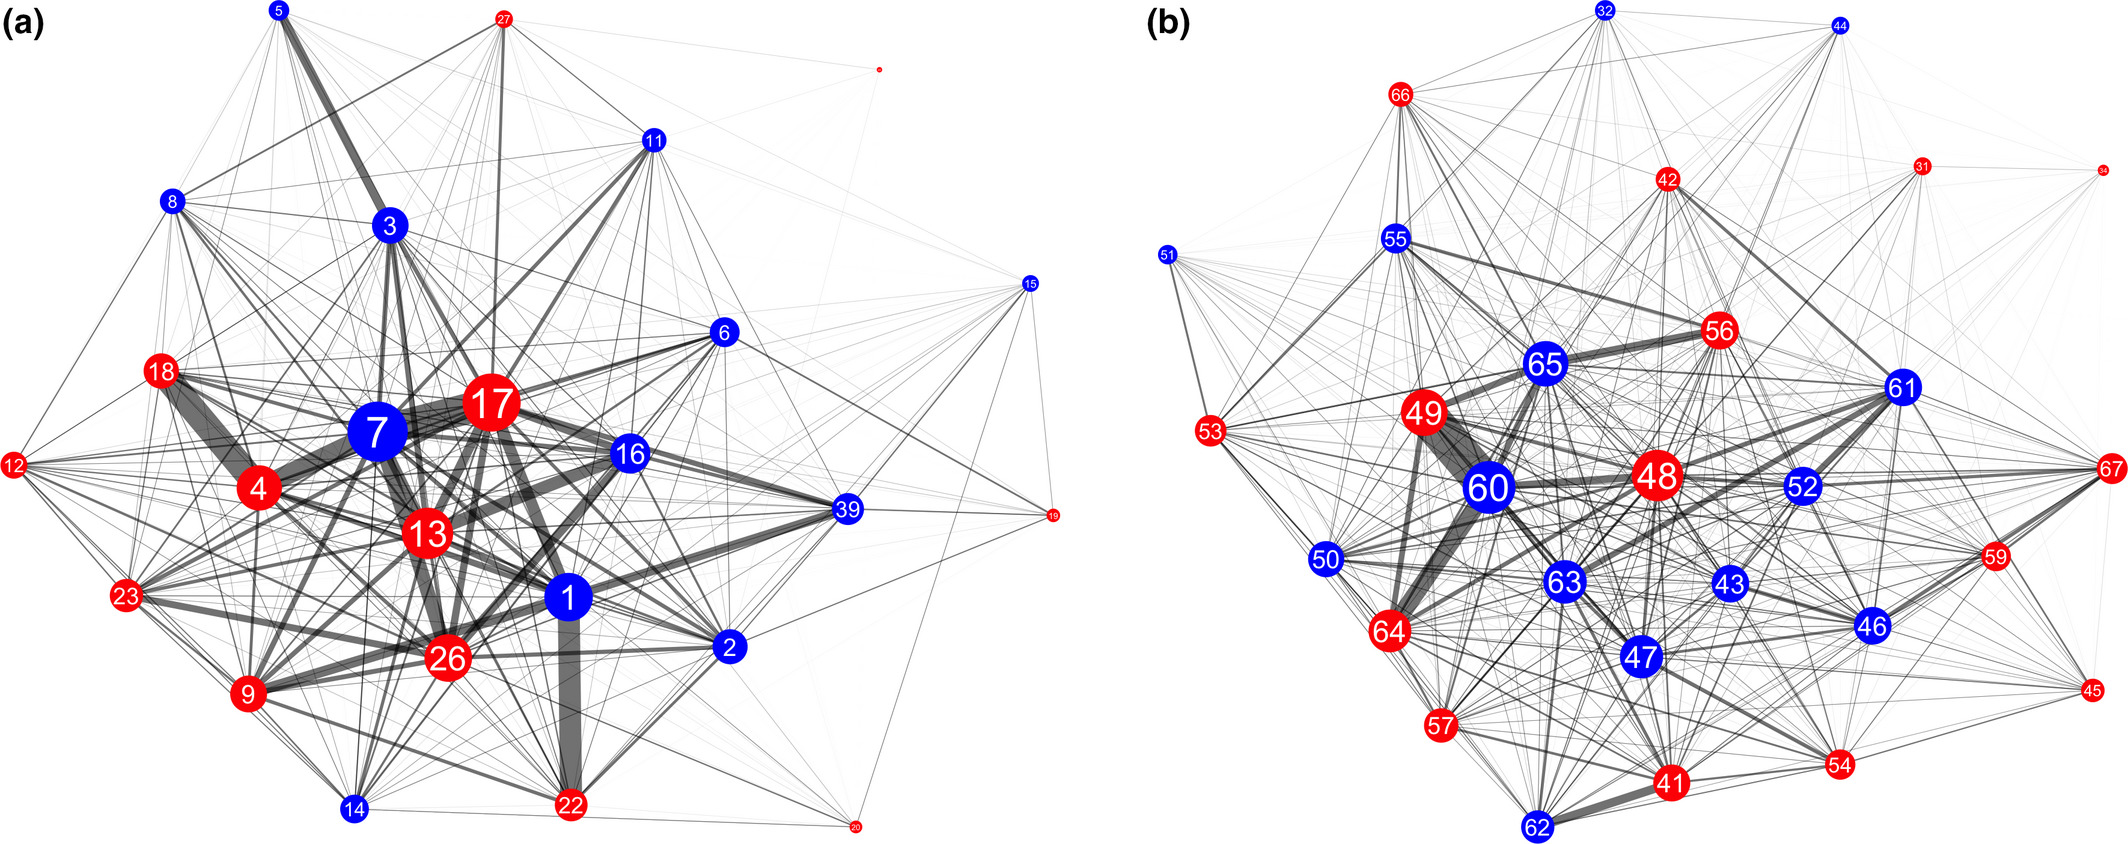
\includegraphics{Graving_IMPRS_Thesis/figures/bird_figure_8.jpg}
    \caption{Affiliative networks generated with co‐feeding data extracted from barcodes detected at a food source using a video camera in (a) flock 1 and (b) flock 2. Each node (circle) represents an individual. Red nodes represent males, and blue nodes represent females. The size of the node represents the individual's degree in the network, a measure of centrality computed by summing the weights of all the edges connected to it. The thickness of the line represents the strength of the association between each pair of individuals
}
    \label{fig:bird_figure_8}
\end{figure}

\subsection{Discussion}
We present a method for recording the behaviour of captive birds using backpack‐mounted barcodes, image capture, and computer detection. With proper deployment, manipulation and monitoring, we have shown that this system is safe for the birds, durable, and capable of delivering extensive data from multiple individuals simultaneously. These position and orientation data can be used to assess multiple types of behaviours, associations and interactions among individuals. This system presents several advantages to more commonly‐implemented methods. In particular, it is adaptable to different contexts and research questions, being possible to vary the temporal resolution (photos or video) and the area covered without requiring any additional markers to birds. For general purposes, the use of Raspberry Pi single‐board computers and camera modules makes this method affordable, enabling high‐throughput data collection that increases sample sizes and statistical power. Our example analyses demonstrate that the barcode‐based approach can generate similar data to what is often collected using PIT tags (Figure 8), but also provides much richer information on movements and spatial location within patches (Figure 7). We found that the backpack system simplified the data analysis because we were certain about the co‐occurrence of birds at the same food source (i.e. captured in the same frame), instead of having to infer co‐occurrences from sequences of detections using pattern‐recognition algorithms (e.g. Psorakis et al., 2015).

We tested the application of different camera setups and behavioural contexts, including video for feeding arenas and photos in co‐perching scenarios. Cameras could be fitted in various locations, including bathing areas, nest boxes, and potentially in open areas to capture birds in flight (e.g. Figure 6). The decision on the type of camera and on video or photos will depend on each research question. For example, researchers could choose video for recording aggressive interactions or other behaviours that involve movement, or capture photos every few seconds to capture affiliative data for the purposes of studying social networks, pair formation, or group stability. The type of data provided by these barcodes also provides new opportunities for analysis. Using machine learning, it will be possible to automatically classify behaviours and interactions over extended periods of time while also minimizing manual annotation by a human observer (Robie, Seagraves, Egnor, & Branson, 2017), thereby avoiding bias and fatigue. Such approaches have been developed for studying other organisms (Kabra, Robie, Rivera‐Alba, Branson, & Branson, 2013), which use data that are similar to what our system generates.

Our backpack‐based barcode method has potential to be extended to diverse range of systems. Although we only collected data during daylight hours, barcodes could easily be detected in low‐light conditions and many commercially available infrared cameras can image the black‐and‐white codes without visible light (using infrared lights). While most birds are not very active at night, there is increasing evidence that many important behaviours happen early in the morning (Bonter, Zuckerberg, Sedgwick, & Hochachka, 2013). Such behaviours could easily be captured with this barcode system but would be almost impossible to study using manual observations or video as it is difficult to identify coloured leg bands. Future applications include using barcodes to identify individuals interacting with a device (e.g. a feeder or a puzzle box). To date, such systems have mostly relied on using PIT tags (e.g. Aplin et al., 2015), which limits sampling to a single individual at once. In social species, individuals often congregate, and a barcode system can facilitate multiple simultaneous detections and quantify relative positions of individuals to one‐another and to the device. The implementation of “real‐time” detection could allow for algorithms that control devices in response to the behaviour of birds, such as allowing only a maximum number of individuals in one area or selectively dispensing food to particular individuals (as performed by Firth, Voelkl, Farine, & Sheldon, 2015). Barcodes could provide a powerful interface between individuals and experimental devices, not only by being able to provide tailored responses (such as individual learning algorithms, Morand‐Ferron, Hamblin, Cole, Aplin, & Quinn, 2015), but also, unlike almost any other system, by capturing information about who else is present when particular events occur.

Although we have discussed the multiple advantages, the limitations of the system must be also considered. While backpacks and barcodes can last for more than 4 months, permanent monitoring was required to assure safety of the birds and adequate delivery of data. Grooming and allopreening caused some wear on the backpacks and codes, and this sometimes led to impaired movement of the birds. Detecting and addressing such issues is important for both safety of the birds and continuity of the data collection. Additionally, there are unavoidable issues that reduce detectability, like fast movement, codes tilted due to extreme body position, and wings or feathers partially covering the trays. The current design of the backpacks addresses these issues well and delivers consistent detection. Additional concerns related to camera systems, such as storage, resolution, lens distortion or lighting, can be solved for specific research circumstances.

A key question that requires further investigation is whether these backpacks will be suitable for field deployment. We found that, in zebra finches, we could detect most issues within the first 1–2 days. However, few field studies are amenable to keeping birds in captivity to allow such monitoring. Thus, field applications may be limited to species that either have well‐established protocols for fitting backpacks in the field or those in which individuals can be easily monitored (e.g. territorial species). We believe that there is a danger that small songbirds could entangle their backpacks in small branches, particularly if backpacks become loose over time. Finally, our aviaries had artificial lighting that remained constant during daytime. Researchers conducting outdoor studies, with natural lighting conditions, must consider the changing environment (i.e. sun position and cloud coverage) to avoid unusable images due to the differences in light quality from dawn/dusk to noon. For example, sun shining directly on the white tag will make the code invisible to the camera, while a setup designed for sunny conditions would create completely black photos under cloudy conditions. The use of infra‐red cameras and infra‐red lighting is one way to overcome this challenge.

Our backpack‐mounted barcode system could revolutionize data collection in a range of experimental systems. We have demonstrated that it can be implemented safely and cheaply. Further, it has the ability to collect extensive data across many individuals simultaneously and the flexibility to address diverse research questions. With simple software modifications, the system can also be integrated into active devices that interface directly with individuals, which will prove to be an extremely powerful experimental approach.

\subsubsection{Data availability}
The raw tracking data files, including the distance from the food patch, that are used for the example data analyses can be found at https://doi.org/10.17617/3.19.




\newpage 
	\section[Chapter 2: DeepPoseKit, a software toolkit for animal pose estimation]{\centering Chapter 2: DeepPoseKit, a software toolkit for fast and robust animal pose estimation using deep learning}
	
	\textbf{Jacob M. Graving, Daniel Chae, Hemal Naik, Liang Li, Benjamin Koger, Blair R. Costelloe, Iain D. Couzin}


\subsection[Nutritional State and Sensory Perception]{The Influence of Nutritional State on Sensory Perception and Group Movement} \label{project2}
\paragraph{Objective:} 
Resolve how nutritional state influences individual sensory perception, decision-making, and group movement
\subsubsection{Background}
Nutritional state can drastically influence the behavior of individuals in groups \citep{lihoreau2015nutritional}. For example, individuals with the highest nutrient requirements are more likely to lead groups \citep{krause1992relationship,fischhoff2007social,mcclure2011group}. In schools of roaches (\textit{Rutilus rutilus}), unfed individuals tend to take front positions \citep{krause1992relationship}, and this position in the group provides them with the highest food intake and a dominant influence on directional decisions of the group \citep{bumann1993front}. In the nomadic forest tent caterpillar (\textit{Malacosoma disstria}), the most protein-deficient individuals initiate collective foraging and lead the group towards new feeding sites, whereas protein-satiated individuals follow behind \citep{mcclure2011group}. Differences in nutritional state among individuals can regulate the emergence of \textit{temporary leadership roles}, where a single individual can determine the movement decisions of the entire group \citep{sumpter2010collective}. 
\par
Nutritional state can also influence sensory perception. For example, when deprived of food, blowflies (\textit{Calliphoridae sp.}) will downregulate activity in their peripheral visual system---presumably to reduce the costs of an energetically expensive sensory system---and increase reliance on energetically cheaper sensory modalities such as olfaction \citep{longden2014nutritional}. Similar changes have been demonstrated in vertebrates as well (reviewed by \citealp{longden2014nutritional}). Additionally, a key assumption of animal communication theory is that receivers dynamically alter their perceptual rules for weighting information modalities depending on relevance, context, and internal state \citep{hebets2016systems}---commonly referred to as \textit{cross-modal perceptual weighting} \citep{stein2012new}, but this assumption is rarely tested explicitly with few notable exceptions (e.g. \citealp{gomes2016bats}).
\par
While the behavioral effects of nutritional state have been studied in locusts \citep{bazazi2011nutritional}, the interacting effects of nutritional state and sensory information have not. \citet{bazazi2011nutritional} showed that protein-deprived locusts move faster when in groups with increased rates of cannibalism, and supplementing locusts with a high-protein diet decreases group movement \citep{bazazi2011nutritional}. However, this study only examined groups with homogeneous nutritional states, and the dynamics of heterogeneous groups remain unstudied. Within heterogenous groups, nutrient-replete individuals should be better able to escape those trying to cannibalize them, as larger energy reserves allow them to move faster for longer \citep{arrese2010insect}. These pursuit and escape responses are mediated by multimodal sensory networks \citep{bazazi2008collective}, and the magnitude, frequency, and modality of sensory stimuli within these networks are a product of other group members' behavior. Movement in response to these sensory stimuli can also influence nutritional state, as faster moving individuals expend more energy, quickly returning to a state of nutrient-deprivation \citep{arrese2010insect} and increasing their motivation to cannibalize others. These heterogeneous autocatalytic dynamics may be comparable to the dynamics of other complex systems (e.g. \citealp{ortega2016visualization,bissette2013mechanisms})
\par
For the sake of theoretical tractability, models of locust marching behavior have also not explicitly, comprehensively, and simultaneously considered many related aspects that may be driving collective movement in locust bands \citep{guttal2012cannibalism,bazazi2011nutritional,romanczuk2009collective}. These aspects include the role of nutritional state in altering the perception and behavior of individuals, the role of individual behavior in altering the movement of others in the group through sensory interaction networks, the role of locomotion in altering nutritional state, and the feedback between these factors and the environment, e.g. the distribution of food resources. Consequently, there exists only a meager theoretical basis for understanding these dynamics.
\par
Past research offers limited understanding of how differences in nutritional state can alter perception, behavior, and the dynamics of group movement. Nutritionally-driven behavioral differences \citep{bazazi2011nutritional} presumably change the magnitude and frequency of visual and tactile interactions between individuals, and while it has been shown that nutritional state alters the decision-making of individuals, it is not precisely understood how these nutritional differences alter sensory perception and internal decision-making rules. None of these questions have been tested explicitly, and here I propose to do so for the first time.


\subsubsection{Methods}

See \ref{sec:methods} for description of experimental setup and general methods.

\paragraph{Experimental Diets}
I will use artificial diets described by Bazazi et al. (2011) to manipulate the nutritional state of individuals. Treatment groups will consist of different mixtures of individuals fed on high- and low-nutrient diets. The exact experimental design will be determined after completion of  \ref{project1} and pilot experiments for \ref{project2}.

\paragraph{Data Analysis}
I will use previously described methods (see \ref{sec:methods}) to compare the perception and behavior of nutritionally-deprived individuals to nutritionally-replete individuals. I will then relate this to the dynamics of collective movement.

\paragraph{Current State}
The barcode tracking, behavioral classification, and visual field reconstruction software packages are all near completion. The experimental setup has been constructed. Final experiments are planned for early 2018.

\subsubsection{Timeline}
\begin{itemize}{}{}
	\item Project duration --- 6 months
	\item Obtaining preliminary results --- 2 months
	\item Obtaining final results --- 2 months	
	\item Final discussion and writing up --- 2 months.
\end{itemize}

\subsection{The Neurobehavioral Dynamics of Group Movement}
\paragraph{Objective:} 
Describe the neurobiological implementation of visually-mediated behavioral programs in locusts and understand how neurophysiological dynamics, such as sensitivity and habituation, affect perception and decision-making of both individuals and collectives.
\subsubsection{Background}
Based on neurophysiology \citep{rind2008arousal,rogers2010spatiotemporal}, loom stimuli created by movement of conspecifics likely contribute significantly to locust marching behavior (reviewed by \citealp{simmons2010escapes}). The largest neurons in locust visual system, the descending contralateral movement detector (DCMD) and lobula giant movement detector (LGMD) (Figure \ref{fig:dcmd}), are highly sensitive to loom stimuli, and there is strong evidence that these neurons are involved in social behaviors. These pathways mediate object avoidance \citep{chan2013collision,gabbiani2002multiplicative} and their activity has been linked to a wide range of collision avoidance behaviors during flight \citep{simmons2010escapes}. Habituation of DCMD to loom stimuli is also five times weaker in gregarious locusts than in solitary locusts \citep{matheson2004plasticity} suggesting that signal transduction by this neuron may be important for social interactions. However, the exact neurophysiological mechanisms of how locusts make decisions in a social context remain almost completely unstudied.
\par
Previous neurophysiological studies of the locust visual system have been primarily limited to tethered experiments with arbitrary visual cues chosen a priori. Instead of making assumptions about which sensory features are relevant to social behavior, I will work backwards by directly immersing a freely behaving locust into a real social context while recording neurophysiological data from the visual system. I will then measure the visual inputs and behavioral outputs using computer vision. Using machine learning methods, I will decompose the relevant visual features, map these features to the features of the recorded neural encoding and map the neural encoding to the behavioral output. This will be the first time all three of these aspects are considered in such a detailed, comprehensive manner and in an ecologically-relevant context. This project will provide new understanding of neurophysiological dynamics of both collective behavior and animal behavior in general.

\subsubsection{Methods}

See \ref{sec:methods} for description of experimental setup and general methods.
\begin{figure}
	\begin{center}
		\includegraphics[width=0.5\textwidth]{dcmdfigure.png}\\
	\end{center}
	\begin{flushleft}
		\caption{In collaboration with others, I will record from the DCMD (\textbf{top}) via the neck connectives (\textbf{bottom}). Figures reproduced from \citealp{berman2013neural,gabbiani2002multiplicative}.  \label{fig:dcmd}} 
	\end{flushleft}
\end{figure} 

\begin{figure}
	\begin{center}
		\includegraphics[width=\textwidth]{electrophysiologyfigure.png}\\
	\end{center}
	\begin{flushleft}
		\caption{Spike sorting using unsupervised machine learning. To better understand how the brain encodes visual information, I have developed software for analyzing electrophysiology traces (\textbf{A}) by automatic spike sorting. Spikes with an amplitude above an automatically determined noise threshold (blue dashed line) are extracted (red spikes, \textbf{B}), embedded into a low-dimensional space (using t-SNE) based on shape (\textbf{C}) and then labeled based on automatic cluster assignment (\textbf{D}) using DBSCAN \citep{ester1996density}. \label{fig:ephys}} 
	\end{flushleft}
\end{figure} 

\paragraph{Neurophysiology}
Collaborating with members of the neurobiology department, I will record from the DCMD via the neck connectives (see \citealp{williamson1982large,berman2013neural} for details) of freely moving locusts interacting with a social group. I will track individual behavior in detail and reconstruct the visual field using the software previously described in \ref{sec:methods}. 

\paragraph{Data Analysis}
Using similar machine learning methods from \ref{sec:methods}, I will relate the visual field to the neural encoding and then relate the neural encoding to the behavioral output (see Figure \ref{fig:ephys} for details).

\paragraph{Current State}
The barcode tracking, behavioral classification, and visual field reconstruction software packages are all near completion. Software for analyzing the electrophysiology data is in development (Figure \ref{fig:ephys}). The experimental setup has been constructed. Electrophysiology rig has been purchased and set up. Recording methods are in development by Angela Albi (PhD student) and Einat Couzin (Principle Investigator). Final experiments are planned for late 2017 - early 2018 depending on the progress with neurophysiology recordings.

\subsubsection{Timeline}
\begin{itemize}{}{}
	\item Project duration --- 6 months
	\item Obtaining preliminary results --- 2 months
	\item Obtaining final results --- 2 months	
	\item Final discussions and writing up --- 2 months.
\end{itemize}


\section{Additional PhD Curriculum}
\subsection{Workshops}
\paragraph{Attended:}
\begin{itemize}
	\item IMPRS Student Retreat 2015
	\item Social Network Analysis
	\item Conference Presentations
	\item Teaching Week
	\item Introduction to GAM and GAMM with R
	\item IMPRS Student Retreat 2016
	\item Introduction to Scientific Writing
\end{itemize}
\paragraph{Plan to Attend:}
\begin{itemize}
	\item Writing Lab for Research Articles
	\item Grant Writing
\end{itemize}
\subsection{Conferences and Symposia}
\paragraph{Attended:}
\begin{itemize}
	\item IMPRS Grand Challenges Symposium 2015: Scientific Communication - Seewiesen, Germany
	\item IMPRS Grand Challenges Symposium 2016: Evolutionary Ecology of Individual Differences - Konstanz, Germany
	\item IMPRS Selection Symposium 2016 - Seewiesen and Konstanz, Germany
	\item European Conference for Behavioural Biology 2016 - Vienna, Austria
	\item ImVis 2017 - Faak am See, Austria
\end{itemize}
\paragraph{Plan to Attend:}
\begin{itemize}
	\item DeepLearn2017 - Bilbao, Spain
\end{itemize}
\subsection{Public Outreach}
\paragraph{Attended:}
\begin{itemize}
	\item Volunteered at \say{Das Schwarmverhalten der Fische}, a public lecture given by Prof. Dr. Jens Krause in Konstanz, Germany
	\item Volunteered at \say{Konstanzer Lange Nacht der Wissenschaften}
\end{itemize}
\paragraph{Plan to Attend:}
\begin{itemize}
	\item Any future scientific communication events organized by the department 
\end{itemize}
\pagebreak


\begin{appendices}
%\pagenumbering{roman}
\begin{figure}
	\begin{center}
		\includegraphics[width=0.3\textwidth]{neuralnetwork.png}\\
	\end{center}
	\begin{flushleft}
		\caption{A simple feed-forward neural network. \label{fig:feedforward}} 
	\end{flushleft}
\end{figure} 

\section{Artificial Neural Networks}  \label{sec:anns}
Artificial neural networks (ANNs) are a class of computational model loosely inspired by biological neural networks in the brain. These models rely on the metaphor of a \textit{computational graph} where a network is represented by a series of interconnected computational \textit{nodes}, also called \textit{neurons}, which form the \textit{layers} of the computational graph. In the simple case of a feed-forward neural network $f: X \to Y$, there is an \textit{input layer} where data $X$ are fed into the network and an \textit{output layer} where the computational output of the network $\hat{Y}$---an estimate of the ground truth $Y$---is produced, and these are connected by one or more \textit{hidden layers} (Figure \ref{fig:feedforward}). As a side note, ANNs are sometimes called \textit{deep neural networks} (DNNs) depending on how many layers of computational nodes they contain, where a network with more than 2 hidden layers is considered \textit{deep}. These hidden layers make up the computational functionality of the graph, with each node of the layer containing parameters known as \textit{weights} and \textit{biases}. Typically the weights and biases of each layer are denoted as a matrix $W^l$ and a vector $\mathbf{b}^l$ respectively, where $l$ is the layer number. At the output of each layer is a function that uses the weights and biases to perform some computation, typically called an \textit{activation}. The activations for the first two hidden layers of a feed-forward ANN are therefore denoted by
\begin{equation}
\begin{aligned}
& \mathbf{a}^1 = h^{1}(W^1\mathbf{x} + \mathbf{b}^1)  \qquad \text{and}\\
& \mathbf{a}^2 = h^{2}(W^2\mathbf{a}^1 + \mathbf{b}^2)\\
& \quad \equiv h^2(W^2h^1(W^1\mathbf{x} + \mathbf{b}^1) + \mathbf{b}^2) 
\end{aligned}
\end{equation}
where $\mathbf{x} \in X$ is the input, and $h^{l}(\cdot)$ is some activation function for layer $l$ (linear, sigmoid, or otherwise). 
\par
The cost function for optimizing these parameters is defined as 
\begin{equation}
C = C(Y,\hat{Y})
\end{equation}
where $C$ is some function penalizing the network output $\hat{Y}$ for being different from the ground truth $Y$. This cost function is then typically minimized, or rather the network is \textit{trained}, through a modified version of gradient descent known as \textit{mini-batch stochastic gradient descent with backpropagation}. In brief, this process is performed in three steps: (1) mini-batches of training data are fed through the network in a forward pass, (2) the error of the output is calculated, and (3) the gradients $\frac{\delta C}{\delta W}$ and $\frac{\delta C}{\delta \textbf{b}}$ are propagated backwards sequentially through the network using the chain rule, updating the parameters $W^l$ and $\mathbf{b}^l$ at each layer $l$. The cost function in the context of this optimization algorithm then takes the form
\begin{equation}
C = \frac{1}{n} \sum_{i=1}^{n} C_i \text{,}
\end{equation}
where $C$ is the average for all cost functions $C_i$ for all $n$ training examples.  
\par
These networks are highly flexible and can be used for everything from image segmentation, object tracking, classification, regression, time-series modeling, and in this case, dimensionality reduction \citep{deeplearningbook}. In fact, there is evidence they can be used to approximate nearly any function or probability distribution \citep{lin2016does}.




\section{Image Registration} \label{sec:imageregistration}
Using the barcode tracking data described in the main text, following \citet{berman2014mapping,berman2014drosopholid} I first generate 200$\times$200px videos of each individual over time. This is accomplished by segmenting the animal from the background and rotationally and translationally aligning each frame to a basis image such that the main trunk of the body is mostly invariant while the limbs are allowed to vary (Figure \ref{fig:alignment}). The details of these alignment algorithms are described elsewhere \citep{berman2014drosopholid,berman2014mapping,de1987registration,reddy1996fft,wilson2006correlation,guizar2008efficient}. Because these images are not lit from behind like the methods described in \citet{berman2014drosopholid,berman2014mapping}, individual color variation can influence the results of the analysis. To solve this, I simply binarize each image such that the pixels describing the body of the animal are white, while the background pixels are black (Figure \ref{fig:convexhull}). 
\par To isolate the pixels describing the behavior of one individual from those describing the behavior of other individuals, I use only those pixels within the convex hull of the pixels with the highest variance (see Figure \ref{fig:convexhull}). This provides a reasonable representation of individual behavior but is still problematic when animals are in very close proximity. This issue has been adequately solved by \citet{klibaite2017unsupervised} for cases where there are only two interacting animals, but this method is unreliable when there are more than two animals interacting. I am currently investigating the use of \textit{fully convolutional neural networks}, a class of ANNs designed for image segmentation \citep{long2015fully}, to produce a higher-quality solution to this problem. After all of these steps, I then utilize these videos as a high-dimensional time-series describing the posture of each individual with a single frame being a feature vector describing the pose at time point $t$, or 
\begin{equation}
X \equiv \{x_1(t),x_2(t),\ldots,x_d(t)\} \text{,}
\end{equation}
where $d$ is the dimensionality of the images. 


\begin{figure}
	\begin{center}
		\includegraphics[width=0.6\textwidth]{alignmentfigure.png}\\
	\end{center}
	\begin{flushleft}
		\caption{The image alignment algorithm. Images are roughly aligned using the vector angle generated from reading the barcode (\textbf{top-left}), segmented from the background such that only the body trunk and rear legs are visible (\textbf{bottom-left}) and then aligned (\textbf{bottom-right}) with a basis image (\textbf{top-right}).  \label{fig:alignment}} 
	\end{flushleft}
\end{figure} 

\begin{figure}
	\begin{center}
		\includegraphics[width=0.8\textwidth]{convexhullfigure.png}\\
	\end{center}
	\begin{flushleft}
		\caption{The convex hull (\textbf{middle}) of high variance pixels (\textbf{left}) used to segment pixels for measuring individual behavior (\textbf{right}).  \label{fig:convexhull}} 
	\end{flushleft}
\end{figure} 



\section{Postural Decomposition} \label{sec:posturaldecomposition}
\paragraph{}
As an insect is composed of a relatively inflexible body segments connected by mobile joints, the number of postural degrees of freedom is much smaller than the current high-dimensional image representation. Following \cite{berman2014mapping,berman2014drosopholid} I then wish to compress this representation to a lower dimensional space while still adequately describing the information contained in the high-dimensional space. \cite{berman2014mapping,berman2014drosopholid} use principal components analysis (PCA) to reduce the dimensionality of images by decomposing the covariance of pixel values into linearly uncorrelated eigenmodes. However, using PCA on large, high-dimensional data sets becomes computationally intractable due to the complexity of the underlying algorithm $O(d^2n+d^3)$, where $d$ is the number of dimensions and $n$ is the number of rows in the data matrix. There are solutions to this problem other than vanilla PCA (e.g. \citealp{rokhlin2009randomized,artac2002incremental}), but these do not provide the flexibility of an ANN and are generally difficult to implement on the GPU. 
\par
Therefore, I have reformulated this step of the framework as an ANN known as a \textit{linear autoencoder}. This implementation has multiple advantages compared to PCA, the most important of which is the ability to train the network online, or out-of-memory, on a GPU using batches of data. Because of this, the overall complexity of the algorithm reduces to low-order polynomial time \citep{magdon2015}. This also allows us to simplify the methods described in \cite{berman2014drosopholid,berman2014mapping}, as we can skip the steps of converting the images to radon space and using only pixel values with the highest variance. Instead, we can directly decompose the high-dimensional images to a low-dimensional representation. 
\par 
In the most general sense, autoencoders are a class of ANNs that seek to copy their inputs to their outputs while minimizing information loss. Autoencoders are defined in the general form $f: X \to Z \to \hat{X}$ \citep{deeplearningbook,hinton2006autoencoder,williams1986learning}. Internally the network architecture has a hidden layer that describes a code $Z$ to represent the input. The network is composed of two parts: an encoder $g: X \to Z$ and a decoder $h: Z \to \hat{X}$ that produces a reconstruction of the input data  (Figure \ref{fig:network}A). The network is then trained to minimize

\begin{equation}
\begin{split}
C(X,\hat{X}) & = C\big(X, f(X)\big) \\
& = C\Big(X, h\big(g(X)\big)\Big) \text{,}
\end{split}
\end{equation}

where $C$ is a cost function penalizing $\hat{X}$ for being dissimilar from $X$, such as mean squared error or cross entropy.
\par
Autoencoder networks are typically designed so that this copying task will result in the encoder $g(X)$ learning some useful description of the data space $X$ rather than simply the identity, i.e. $X \neq g(X) = Z$. One way to achieve this is to create a bottleneck in the network by constraining $Z$ to a lower-dimensional space than $X$. Learning this lower-dimensional representation forces the autoencoder to capture the most important features of the data. Subsequently, when the decoder $h(Z)$ is \textit{linear} and $C$ is the \textit{mean squared error}, the encoder $g(X)$ will learn to span the same subspace as PCA, i.e.  minimizing information loss of the reconstruction $\hat{X}$ maximizes variance explained by the encoded space $Z$ \citep{deeplearningbook}. In this sense, PCA is the optimal linear autoencoder with respect to global information loss (see \citealt{magdon2015} for details). In practice, linear autoencoders can only achieve near-PCA performance, but this is adequate for my purposes. 

\par
To perform linear decomposition of rotationally and translationally aligned images, I define a feed-forward neural network $f: X \to Z \to \hat{X}$. The network is composed of an encoder $g: X \to Z$ that maps input images $X$ to the latent space $Z$ and a decoder $h: Z \to \hat{X}$ that then maps the encoding $Z$ to a reconstruction of the original image $\hat{X}$. For ease of explanation, I will temporarily relax the computational graph metaphor of a neural network. More formally, the data matrix is $X \in \mathbb{R}^{n \times d}$ (each row $x_i^{T} \in \mathbb{R}^{1 \times d}$ is a data point in $d$-dimensions). The autoencoder is then a pair of linear mappings
\begin{align}
& g: \mathbb{R}^d \mapsto \mathbb{R}^k \qquad  \text{and}\\
& h: \mathbb{R}^k \mapsto \mathbb{R}^d \text{,}
\end{align}
where $k < d$, specified by an encoder matrix $G \in \mathbb{R}^{d \times k}$ and a decoder matrix $H \in \mathbb{R}^{k \times d}	$. For each data point $\mathbf{x} \in \mathbb{R}^d$, the encoded feature vector is defined as
\begin{equation}
\mathbf{z} = g(\mathbf{x}) = G^{T}\mathbf{x} \in \mathbb{R}^k
\end{equation}
and the reconstruction is
\begin{equation}
\mathbf{\hat{x}} = h(\mathbf{z}) = H^{T}\mathbf{z} \in \mathbb{R}^d \text{.}
\end{equation}
Using $\hat{X} \in \mathbb{R}^{n \times d}$ to denote the reconstructed data matrix, I then have
\begin{equation}
\hat{X} = XGH \text{.}
\end{equation}
Returning to the neural network metaphor, the output of the autoencoder network $f: X \to Z \to \hat{X}$ is subsequently defined as
\begin{equation}
\hat{X} = XW^{l-1}W^l
\end{equation}
where $W$ is a matrix of weights for a single layer and $l$ is the total number of layers in the network ($l=2$ in this case).
Importantly, this implementation lacks any bias vectors, i.e.
\begin{equation}
\hat{X} = XW^{l-1}W^l = W^l(XW^{l-1}+\mathbf{b}^{l-1}) + \mathbf{b}^{l} \text{,}
\end{equation}
which enforces orthogonality in the latent space---a desirable property if the goal is to match the results of PCA \citep{konda2014zero}. 
\par
Because PCA is also typically performed on centered and scaled data (i.e. on the covariance or correlation matrix respectively), I also add a batch normalization, or \textit{batch norm}, layer between the input and the encoder layer. Batch norm is a layer commonly used for artificial neural networks to maintain activations at zero mean and unit variance, thereby speeding up convergence \citep{ioffe2015batch}. Here I use it to center the input data such that 
\begin{equation}
\hat{X} = \mathit{BN}_{\gamma,\beta}(X)W^{l-1}W^l \text{,}
\end{equation}
where $\mathit{BN}_{\gamma,\beta}(\cdot)$ is the batch norm function with learnable parameters $\gamma$ and $\beta$ for scale and shift respectively. The batch norm layer performs the computation
\begin{equation}
a_i = \mathit{BN}_{\gamma,\beta}(x_i)  \equiv \frac{\gamma (x_i - \mu)}{\sqrt{\sigma^2+ \epsilon}} + \beta 
\end{equation}
where $a_i$ is the output of the batch norm layer for mini-batch $x_i \in X$, $\epsilon$ is a small number added to avoid division by zero, $\mu$ is the mini-batch mean
\begin{equation}
\mu = \frac{1}{m} \sum_{i=1}^{m}x_i\text{,}
\end{equation}
 and $\sigma^2$ is the mini-batch variance
 \begin{equation}
 \sigma^2 = \frac{1}{m} \sum_{i=1}^{m}(x_i-\mu)^2 \text{.}
 \end{equation}
In this case, I am only interested in centering the data. Therefore, I parameterize the batch norm layer such that such that 
\begin{equation}
a_i = \mathit{BN}_{\beta}(x_i) \equiv x_i -  \mu + \beta  \text{.} 
\end{equation}
\par
Now that the details of the network design are clear, the cost function for training the network is defined as 
\begin{equation}
C = \mathit{MSE}(X,\hat{X}) \equiv \frac{1}{n} \sum_{i=1}^{n} \norm{\mathbf{\hat{x}}_i -\mathbf{x}_i}^2 \text{.}
\end{equation}

The minimization of the cost function $C$ can be performed, like any other feed-forward neural network, by mini-batch stochastic gradient descent with backpropagation---using any of a number of learning algorithms now commonplace in the machine learning literature (reviewed by \citealt{ruder2016}). 
\par
After training, the decoder $h(Z)$ is discarded, and the data matrix $X \in \mathbb{R}^{n\times d}$ is transformed with the encoder $g(X)$ into the latent space $Z  \in \mathbb{R}^{n\times k}$ to reduce the dimensionality from $d$ to $k$. $Z$ is then a linearly-compressed $k$-dimensional description of posture at each time point with each dimension representing a mode of variation within the postural space, or 
\begin{equation}
Z \equiv \{z_1(t),z_2(t),\ldots,z_k(t)\} \text{.}
\end{equation}

\par
The question then remains, how to set $k$ for dictating the dimensionality of the latent space. \cite{berman2014mapping,berman2014drosopholid} chose to use 50 eigenmodes based on the finite sampling error of the data, which is determined by performing PCA on a shuffled data matrix. This choice is complicated by the fact that, unlike PCA, a linear autoencoder is a sub-optimal solution for linear compression. I find that the results of the final behavioral mapping are qualitatively invariant to the choice of $k$, provided it is large enough. Since most of the intensive computation has been moved to the GPU, increasing the dimensionality of this step does not drastically affect computation time for the rest of the pipeline, but it does indeed have an effect. Currently, I am using $k=$ 200, but the effects of this hyperparameter on the quality of the final embedding need to be explored more rigorously to find an optimal value. 
\par
Unlike \citet{berman2014drosopholid,berman2014mapping} I find that parts of this compressed description are directly interpretable. By visualizing the encoder weights of each postural mode, I find that the three modes with the largest encoder weights (comparable to the first three eigenmodes from PCA) are describing postures related to typical tripod-gait locomotion as well as the positions of the rear legs corresponding to left and right turns (Figure \ref{fig:posture}). The remaining postural modes are not as easily interpretable, which is likely due to the nonlinear topology of the postural space.

\begin{figure}	
	\begin{center}
		\includegraphics[width=1\textwidth]{posturefigure.png}\\
	\end{center}
	\begin{flushleft}
		\caption{A visualization of the three postural modes with the largest encoder weights (ordered from left to right). When values for these modes are positive limbs are in the red locations, and when values are negative limbs are in the blue locations (see Figure \ref{fig:spectrogram}).\label{fig:posture}} 
	\end{flushleft}
\end{figure} 

\section{Spectrogram Generation}  \label{sec:spectrogramgeneration}
The instantaneous values of the postural modes do not provide a complete description of behavior, as the definition of stereotypy within this framework is intrinsically dynamical. Within this postural space, it is challenging to recognize behaviors that correspond to similar sequences of movements especially considering the possibility that limbs can move at different times and with different durations. To solve this, I  follow \cite{berman2014mapping,berman2014drosopholid} to generate spectrograms of the postural modes $z_k(t)$. Using a Morlet continuous wavelet transform, I calculate the power spectrum $S(k,f;t)$ for each mode $k$. I also use a dyadically-spaced set of frequencies between $f_{min} = 1$ Hz and the Nyquist frequency ($f_{max} = 45$ Hz) via
\begin{equation}
f_i = f_{max}2^{\frac{i-1}{N_{f}-1}log_2\frac{f_{max}}{f_{min}}}
\end{equation}
for $i = 1, 2, \ldots , N_f$. $S(k,f;t)$ is comprised of 25 frequencies for each of the 200 postural modes, making each point in time represented by a 5000-dimensional feature vector. The feature vector at each time point is then a description of changes in posture over multiple timescales, which will now be referred to as the postural dynamics space, or simply the behavioral space.

\begin{figure}
	\begin{center}
		\includegraphics[width=0.7\textwidth]{spectrogramfigure.png}\\
	\end{center}
	\begin{flushleft}
		\caption{A spectrogram (\textbf{top}) of the first postural mode (\textbf{bottom}), which describes locomotion related postures (see Figure \ref{fig:posture}). Note the characteristic frequency of locomotion. \label{fig:spectrogram}} 
	\end{flushleft}
\end{figure} 

\section{Spatial Embedding} \label{sec:spatialembedding}

Given that the dynamics of the behavioral space likely do not fill the current 5000-dimensional parameterization, I now seek to reduce the dimensionality of this representation in a way that preserves the local neighborhood relationships. \citet{berman2014mapping,berman2014drosopholid} use t-distributed stochastic neighbor embedding (t-SNE) to map high-dimensional behavioral feature vectors into a low-dimensional embedding as a way to capture the most important features of the dataset. Like all dimensionality reduction techniques, t-SNE maps a high-dimensional space to a low-dimensional space while preserving a set of invariants. t-SNE was chosen for this step as it reduces dimensionality by distorting the distances between more distant points while preserving distances between nearby neighbors with minimal local distortion.
\par
I have reformulated this step of the framework as a DNN known as parametric t-SNE. Similar to replacing PCA with a linear autoencoder, this reduces the computational complexity of the algorithm to low-order polynomial time. I largely follow the methods introduced by Van der Maaten and Hinton (2008) and Van der Maaten (2009)---with modifications following Berman et al. (2014)---to train a feed-forward neural network to learn the parametric mapping $f: X \to Y$ between a high-dimensional data space X and the low-dimensional latent space Y (Figure \ref{fig:network}). 
\par
To achieve this, pairwise distances $d(t_i,t_j)$ (yet undefined) are calculated between each time point $i$ and $j$. The distances are transformed into probabilities by centering an isotropic Gaussian over each time point $i$, computing the density of time point $j$, and renormalizing, yielding the conditional probabilities $p_{j|i}$
\begin{equation}
p_{j|i}= \frac{exp(-d(t_i,t_j)^2/2\sigma^2_i)}
{\sum_{k\neq i} exp(-d(t_i,t_k)^2/2\sigma^2_i)}.
\end{equation}
The conditional probabilities are then symmetrized to form a single joint distribution
\begin{equation}
p_{ij} = \frac{(p_{j|i} + p_{i|j})}{2n},
\end{equation}
and the joint probabilities $p_{ij}$ are then a measure of similarity between time points $i$ and $j$.
\par
To measure the pairwise similarity of time points $i$ and $j$ in the latent space, a symmetric distribution, which for technical reasons is a heavy-tailed Student-t distribution (van der Maaten, 2009; van der Maaten, 2008), is centered over each time point $i$ in the latent space. Again, the density of time point $j$ under this distribution is measured and the result is renormalized to obtain joint probabilities $q_{ij}$. The mapping from the data space to the latent space is defined by the feed-forward neural network as $f: X \to Y$, therefore we define $q_{ij}$ as
\begin{equation}
q_{ij} = \frac{(1+\norm{(t_i|W)-f(t_j|W)}^2/\alpha)^{-\frac{\alpha + 1}{2}}}{\sum_{k\neq l}(1+\norm{(t_k|W)-f(t_l|W)}^2/\alpha)^{-\frac{\alpha + 1}{2}}},
\end{equation}
where $W$ is the weights of the network, $f(t_i|W)$ is the activations from the output layer for each time point $i$, and $\alpha$ is the number of degrees of freedom for the Student-t distribution. In my implementation, $\alpha$ is set as $\alpha = d -1$, as described by Van der Maaten (2009), where $d$ is the dimensionality of the latent space.
\par
The weights of the parametric t-SNE network are learned such that the Kullback-Leibler (KL) divergence between the two joint probability distributions $P$ and $Q$ is minimized. This is achieved by minimizing
\begin{equation}
C = D_{KL}(P||Q) \equiv \sum_{i\neq j}p_{ij}log\frac{p_{ij}}{q_{ij}}
\end{equation}
As with the autoencoder network, the minimization of the cost function $C$ can be performed by mini-batch stochastic gradient descent with backpropagation. See \citet{vandermaaten2009ptsne} for further details on the computation of the backpropagation gradients for training the network.
\par
Lastly, I define the distance function $d(t_i,t_j)$ between feature vectors for time points $i$ and $j$. I follow \citealt{berman2014drosopholid,berman2014mapping} by first normalizing each behavioral feature vector
\begin{equation}
\hat{S}(k,f;t) = \frac{S(k,f;t)}{\sum_{k',f'}S(k',f';t)'}
\end{equation}
and then defining the distance function as the KL divergence between feature vectors
\begin{equation}
\begin{split}
d(t_i,t_j) & = D_{KL}(t_i||t_j) \\
& \equiv \hat{S}(k,f;t_i)log_2\bigg[\frac{\hat{S}(k,f;t_i)}{\hat{S}(k,f;t_j)}\bigg]
\end{split}
\end{equation}

After training the network, I then transform the data matrix $S(k,f;t)$ to the embedded space $Y$, estimate the underlying probability distribution using 2-D kernel density estimation, and segment the density peaks using a watershed transform. Preliminary results of this embedding are shown in Figure \ref{fig:embedding}. These results were generated using a limited data set of a 30-minute video of one individual ($n_{frames}\approx 162,000$). The results look promising, but more data are needed to fully assess the quality of the analysis.

\begin{figure}
	\begin{center}
		\includegraphics[width=0.75\textwidth]{neuralnetworkfigure.png}\\
	\end{center}
	\begin{flushleft}
		\caption{A network diagram of an autoencoder (\textbf{A}) and parametric t-SNE (\textbf{B}). Figures reproduced from \citet{hinton2006autoencoder} and \citet{vandermaaten2009ptsne}.\label{fig:network}} 
	\end{flushleft}
\end{figure} 

\begin{figure}
	\begin{center}
		\includegraphics[width=\textwidth]{embeddingfigure.png}\\
	\end{center}
	\begin{flushleft}
		\caption{Preliminary results of spatial embedding (\textbf{left}), kernel density estimation (\textbf{middle}), and watershed segmentation (\textbf{right}). Manually labeled behaviors are marked by colored trajectories through behavioral space (\textbf{left}) where \textit{red} corresponds to locomotion, \textit{blue} corresponds to anterior movement (antennal movement), \textit{green} corresponds to posterior movement (the movement of the rear legs), and \textit{yellow} corresponds to stationary behavior with a brief bout of single leg movements.  \label{fig:embedding}} 
	\end{flushleft}
\end{figure} 


\end{appendices}

\pagebreak
\bibliographystyle{apacite}
\addcontentsline{toc}{section}{References}
\bibliography{Graving_IMPRS_PhD_Proposal_Bib.bib}

\section{Acknowledgements}

\paragraph{Chapter 1}
We thank Jana Hörsch, Laila Darouich, Alex Bruttel, Daniel Zuñiga and the animal caretaker team at the Max Planck Institute for Ornithology in Radolfzell for assistance with data collection and monitoring animal health each day. We thank Iain Couzin, Andrew Straw and two anonymous reviewers for helpful comments on the manuscript. We also thank Iain Couzin for his support of the project. This work was funded by the Max Planck Society. D.R.F. and A.A.M.‐C. received additional funding from the German Research Foundation (DFG grant FA 1420/4‐1 awarded to D.R.F.).

\section{Author Contributions}
\paragraph{Chapter 1}
D.R.F. conceived the project; G.A.‐N. and J.A.K.‐I. developed the backpack design and deployment procedure; IM monitored the health of the birds and impacts of the backpacks; G.A.‐N. tested image and video capture methods, and collected the data; J.M.G. developed the pinpoint software and assisted with the design of the image and video capture methods; A.A.M.‐C. and J.A.K.‐I. performed the example data analyses; G.A.‐N. and D.R.F. wrote the first draft of the manuscript. All authors contributed to editing and revising the final manuscript.

\end{document}